\documentclass[a4paper]{article}

%% Language and font encodings
\usepackage[french]{babel}
\usepackage[utf8x]{inputenc}
\usepackage[T1]{fontenc}

%% Sets page size and margins
\usepackage[a4paper,top=3cm,bottom=3cm,left=2cm,right=2cm,marginparwidth=2cm]{geometry}
%% Useful packages
\usepackage{amsmath}
\usepackage{graphicx}
\usepackage[colorinlistoftodos]{todonotes}
\usepackage[colorlinks=true, allcolors=black]{hyperref}
\usepackage{fourier-orns}
\usepackage{titlesec}
\usepackage{fancyhdr}
\usepackage{fancyvrb}
%\renewcommand{\thefootnote}{\*}
\pagestyle{fancy} 
\setcounter{tocdepth}{5}
\usepackage{float}


%% Tikz stuff
\usepackage{tikz}
\usetikzlibrary{calc, arrows}
\tikzstyle{incolore} = [rectangle, rounded corners, draw=black, minimum height=1cm, minimum width=3cm, text width=3cm, text centered]


%% Pour les exemples
\usepackage{mdframed}
\newmdenv[topline=false, bottomline=false, rightline=false, skipabove=\topsep, skipbelow=\topsep]{example}


\usepackage{libertine}
\newcommand{\hsp}{\hspace{20pt}}
\newcommand{\HRule}{\rule{\linewidth}{0.5mm}}


\renewcommand{\headrulewidth}{1pt}
\fancyhead[C]{} 
\fancyhead[L]{}
\fancyhead[R]{\footnotesize{\leftmark}}

\renewcommand{\footrulewidth}{1pt}
\fancyfoot[C]{} 
\fancyhead[L]{}
\fancyfoot[R]{\thepage}

\definecolor{Zgris}{rgb}{0.87,0.85,0.85}

\usepackage{eso-pic,graphicx}
\usepackage{xcolor}
\newcommand{\bgimg}[1]{
\AddToShipoutPicture
   {
      \put(\LenToUnit{0 cm},\LenToUnit{0 cm})
      {
            \includegraphics[width=\paperwidth,height=\paperheight]{#1} 
      }
   }
}
\begin{document}




%%\bgimg{Image_15.jpg}

















\begin{titlepage}
  \begin{sffamily}
  \begin{center}
    % Upper part of the page. The '~' is needed because \\
    % only works if a paragraph has started.
    
\includegraphics[width=5cm]{LogoHenallux.PNG}~\\[1.5cm]
    \textsc{\Large Rapport de laboratoire}\\[1.5cm]
    % Title
    \HRule \\[0.4cm]
    { \huge \bfseries Troisième laboratoire: Analyse de signaux\\[0.4cm] }
    \HRule \\[2cm]
    % Author and supervisor
    \begin{minipage}{0.4\textwidth}
      \begin{flushleft} \large
        Roumache Grégoire\\
        Sénéchal Julien\\
        Robert Alexandre\\
        Wallemme Maxime\\
        Kenmeugne Lionel\\
        Didion Charles
      \end{flushleft}
    \end{minipage}
    \begin{minipage}{0.55\textwidth}
      \begin{flushright} \large
    	Laboratoire de sciences appliquées à l'informatique\\
		Sécurité des systèmes, technologie de l'informatique\\
		Première année, groupe H \\
		Hénallux\\
		Année académique 2019-2020\\
      \end{flushright}
    \end{minipage}
    \vfill
    % Bottom of the page
    {\large 12 Mars 2020}
  \end{center}
  \end{sffamily}
\end{titlepage}







\let\cleardoublepage\clearpage















\section{Introduction}





Ce troisième laboratoire de sciences appliquées porte sur l'analyse de signaux électriques. Ces signaux sont générés par un générateur de fonctions et analysées par deux appareils, un appareil spécialisé, l'oscilloscope et un appareil plus général, le multimètre. Nous commencerons ce rapport par un rappel théorique des grandeurs électriques et les relations qui les lient entre elles ainsi qu'une brève explication du fonctionnement des appareils utilisés et en particulier les fonctions dont nous avons eu besoin pour le bon déroulement de l'expérience.















\section{Rappels théoriques}










\subsection{Quelques grandeurs électriques}





Afin de mieux comprendre les mesures que nous réalisons, il convient de rappeler quelques grandeurs électriques:
\begin{itemize}
    \item La \textbf{pulsation} est, pour un phénomène périodique, la vitesse de rotation (vitesse angulaire) qu'aurait un système rotatif de même fréquence. Elle est donnée par: $ \omega = 2 \pi f $, et son unité est le radian par seconde.
    \item La \textbf{fréquence} est la mesure du nombre de fois qu'un phénomène périodique se produit en une seconde.
    \item Pour un phénomène périodique, l'\textbf{amplitude} est la grandeur maximale que prend ce phénomène par rapport à sa médiane, pour un signal périodique donné par: $ A \sin (\omega t + \phi) $, on trouve que \textit{A} est l'amplitude du signal.
    \item La \textbf{tension} est mesurée en volts et représente, dans un circuit électrique, la circulation du champs électrique. Pour une résistance qui reste constante au fil du temps, la tension est proportionnelle à l'intensité du courant électrique. \\
    Dans un courant alternatif sinusoïdal, il y a plusieurs tensions spécifiques que l'on peut mesurer, elles sont illustrées sur le schéma de la figure \ref{fig:differentsTension}.

    \begin{figure}%[H]
      \centering
      \begin{tikzpicture}
        \draw [->] (0,-1.2) -- (0,1.2);
        \draw [->] (0,0) -- (3.30,0);
        \draw [thick, domain=0:pi] plot (\x,{sin(\x r * 2)});
        
        \draw[<->] (3.5,1) -- node[anchor=west]{$V_{cc}$ = tension crête à crête} (3.5,-1);
        \draw[<->] (-0.25,0) -- node[anchor=east]{tension de crête = $V_{c}$} (-0.25,1);
        \draw[dashed] (0,0.7071) -- (3.75,0.7071) node[anchor=west]{$V_{eff}$ = tension efficace};
      \end{tikzpicture}
      \caption{Schéma montrant les différents types de tension}
      \label{fig:differentsTension}
    \end{figure}
    \textbf{Remarque}: la tension efficace est donnée, dans ce cas-ci par:
    \[ V_{eff} = \frac{V_c}{\sqrt{2}} \]
    \item Le \textbf{décibel} en électricité est utilisé pour mesurer le gain d'un signal. Dans notre cas, ce sera l'amplificateur du générateur de fonction qui réduira la puissance du signal de 20 dB. Le gain est donné par la relation:
    \[ G_{dB} = 10 \log \frac{P_S}{P_E} \]
    où $P_E$ est la puissance du signal qui entre dans l'amplificateur et $P_S$ est la puissance du signal de sortie.
\end{itemize}










\subsection{Fonctions des appareils utilisés}





Les appareils utilisés pour générer et mesurer le courant électrique sont les suivants:
\begin{itemize}



\item Le \textbf{générateur de fonctions} sert à générer un courant alternatif qui peut être sinusoïdal, carré ou triangulaire. Il permet aussi de contrôler la fréquence, l'amplitude et l'offset du signal. Il est représenté sur la figure \ref{fig:generateurFonction}.

\begin{figure}%[H]
    \centering
    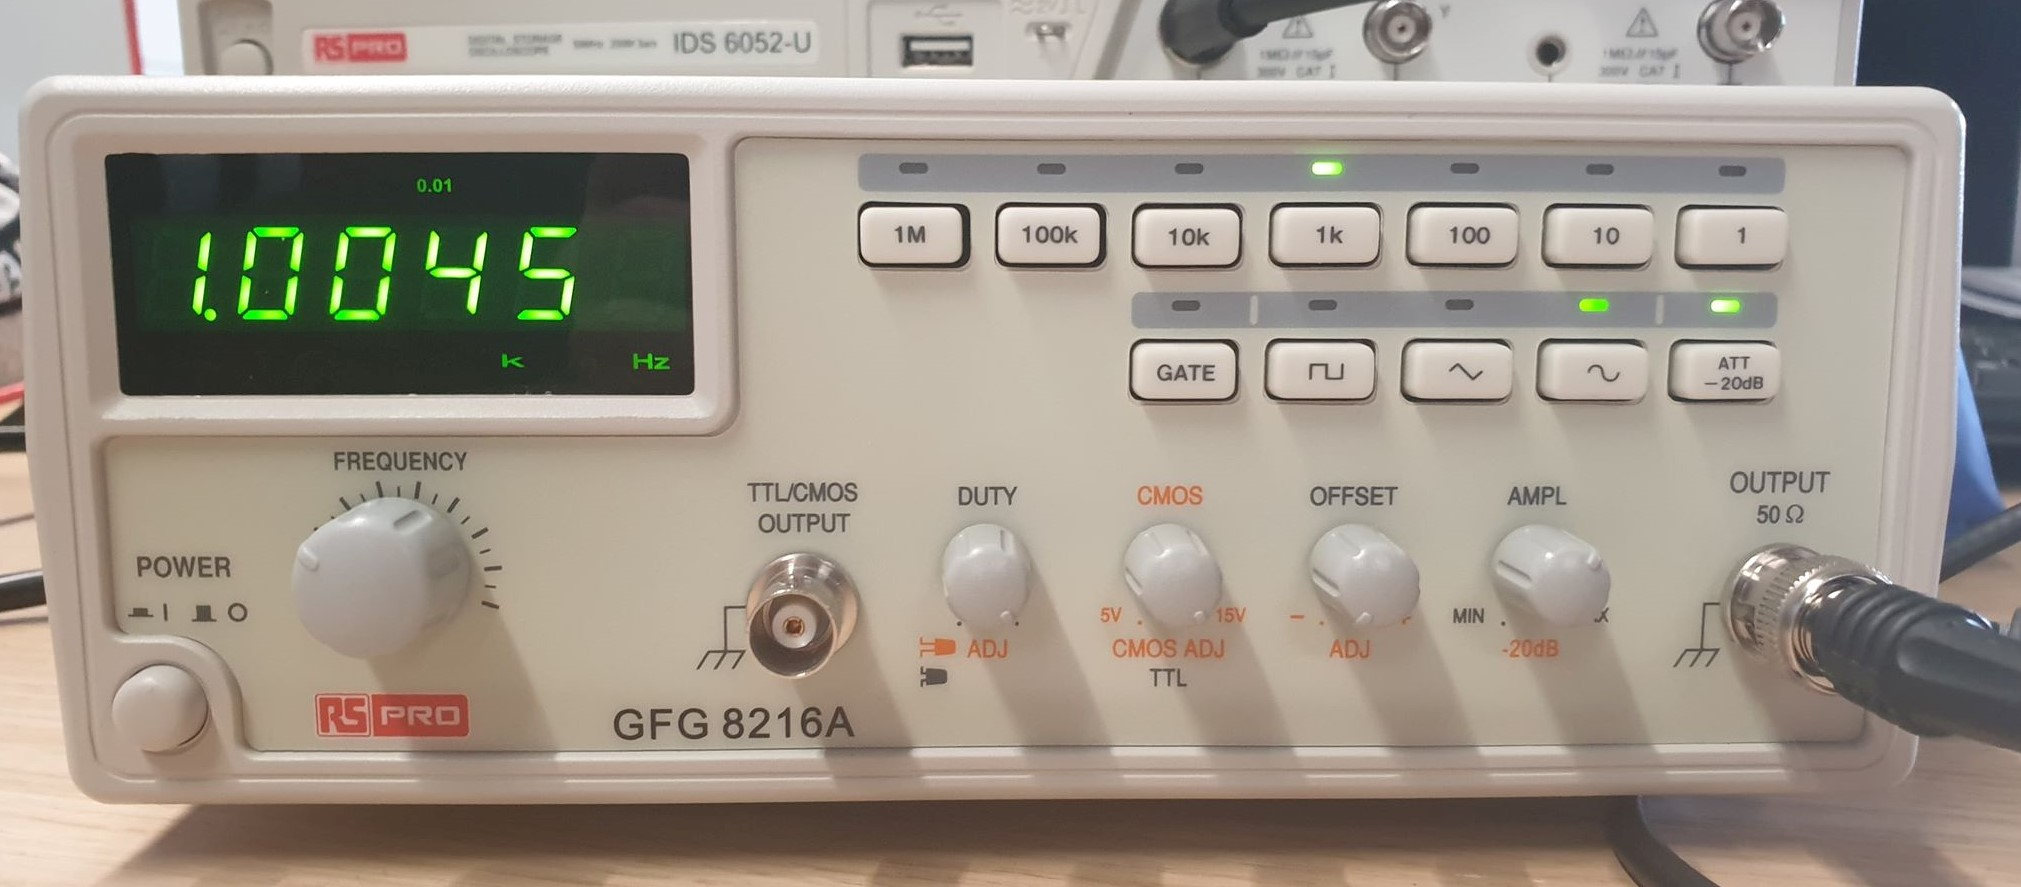
\includegraphics[width=0.85\textwidth]{generateur-fonction01.jpg}
    \caption{Générateur de fonctions}
    \label{fig:generateurFonction}
\end{figure}



\item L'\textbf{oscilloscope} est un outil de mesure de courant électriques alternatifs, autrement dit des courant électriques qui oscillent. Il est représenté sur la figure \ref{fig:oscilloscope}.

\begin{figure}%[H]
    \centering
    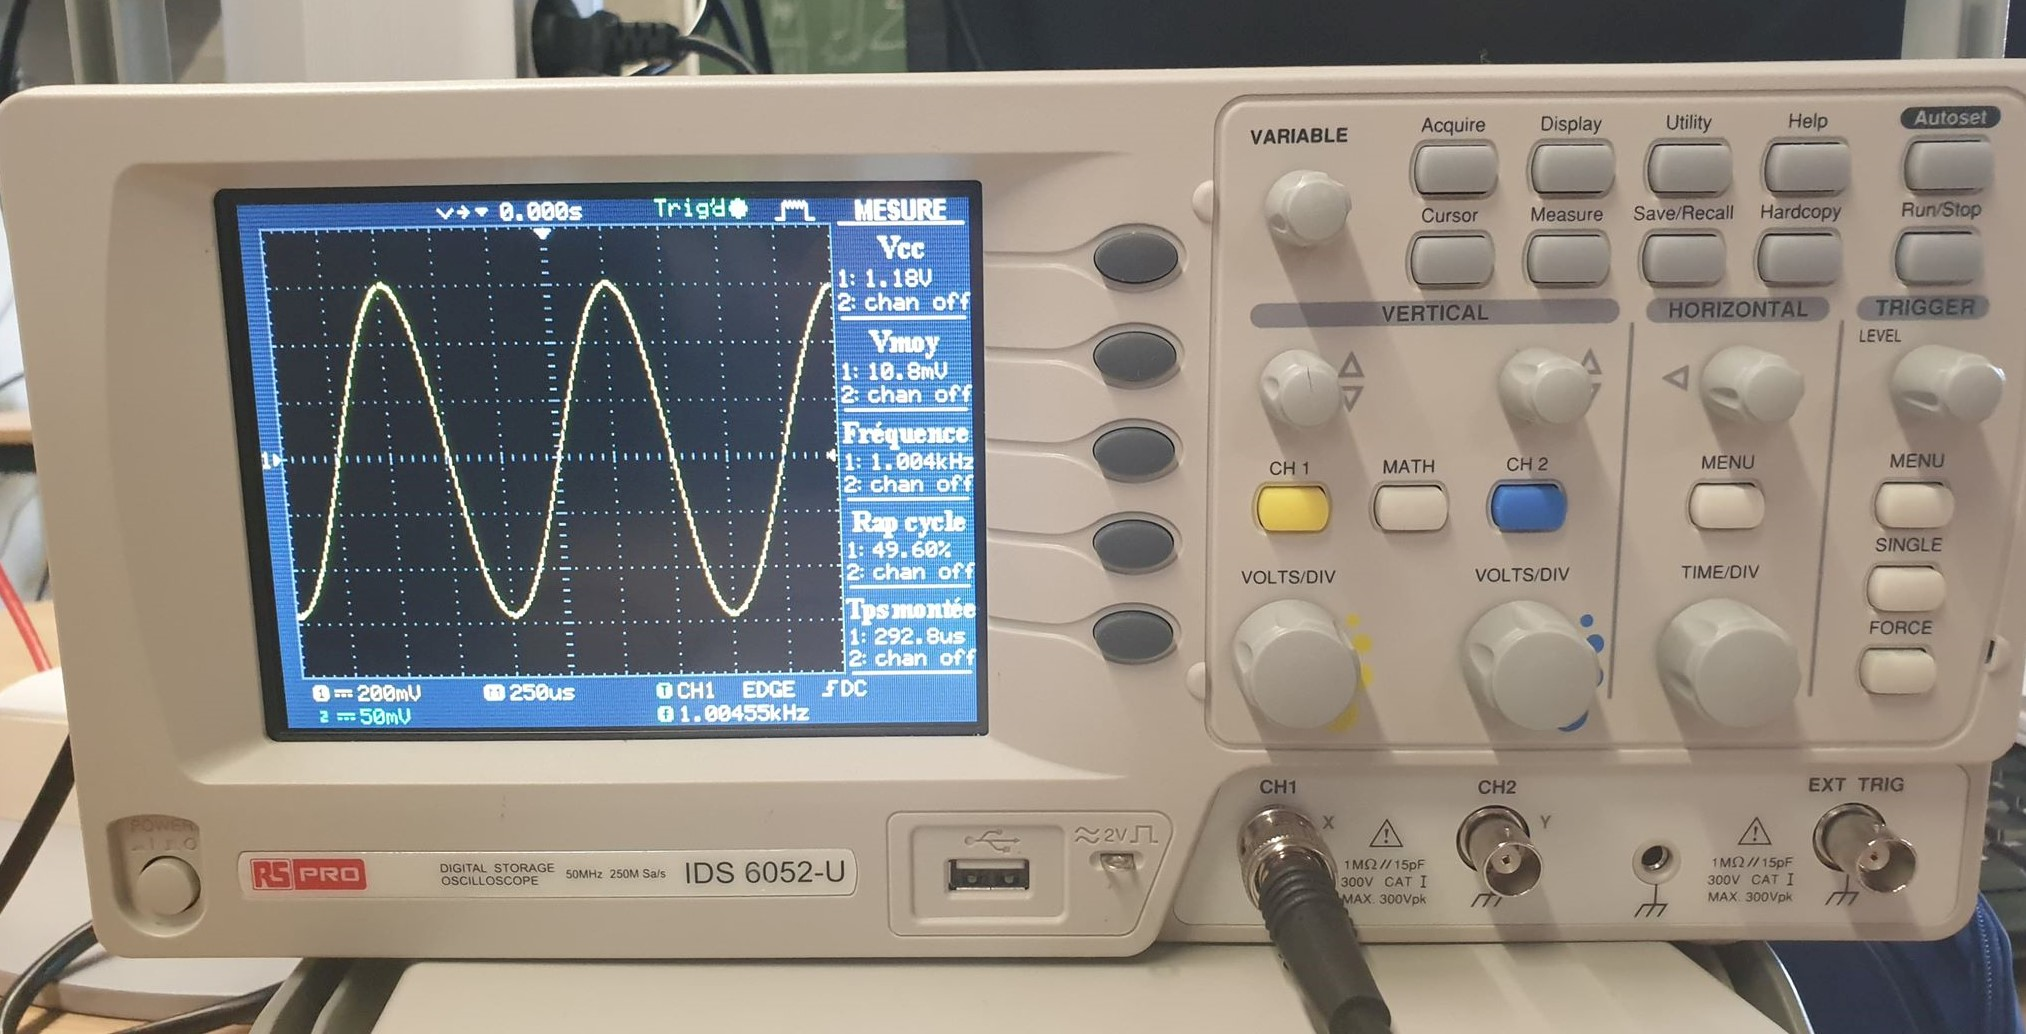
\includegraphics[width=0.85\textwidth]{oscilloscope01.jpg}
    \caption{Oscilloscope}
    \label{fig:oscilloscope}
\end{figure}



\item Le \textbf{multimètre} est un outil de mesure qui fait à la fois voltmètre, ampèremètre et ohmmètre. Il est représenté sur la figure \ref{fig:multimetre}.\footnote{Source de l'image: \texttt{https://www.amazon.fr/Eventek-Multim\%C3\%A8tre-Num\%C3\%A9rique-Portable} \\ \texttt{-R\%C3\%A9tro\%C3\%A9clair\%C3\%A9/dp/B07GSTZL1F}}

\begin{figure}%[H]
    \centering
    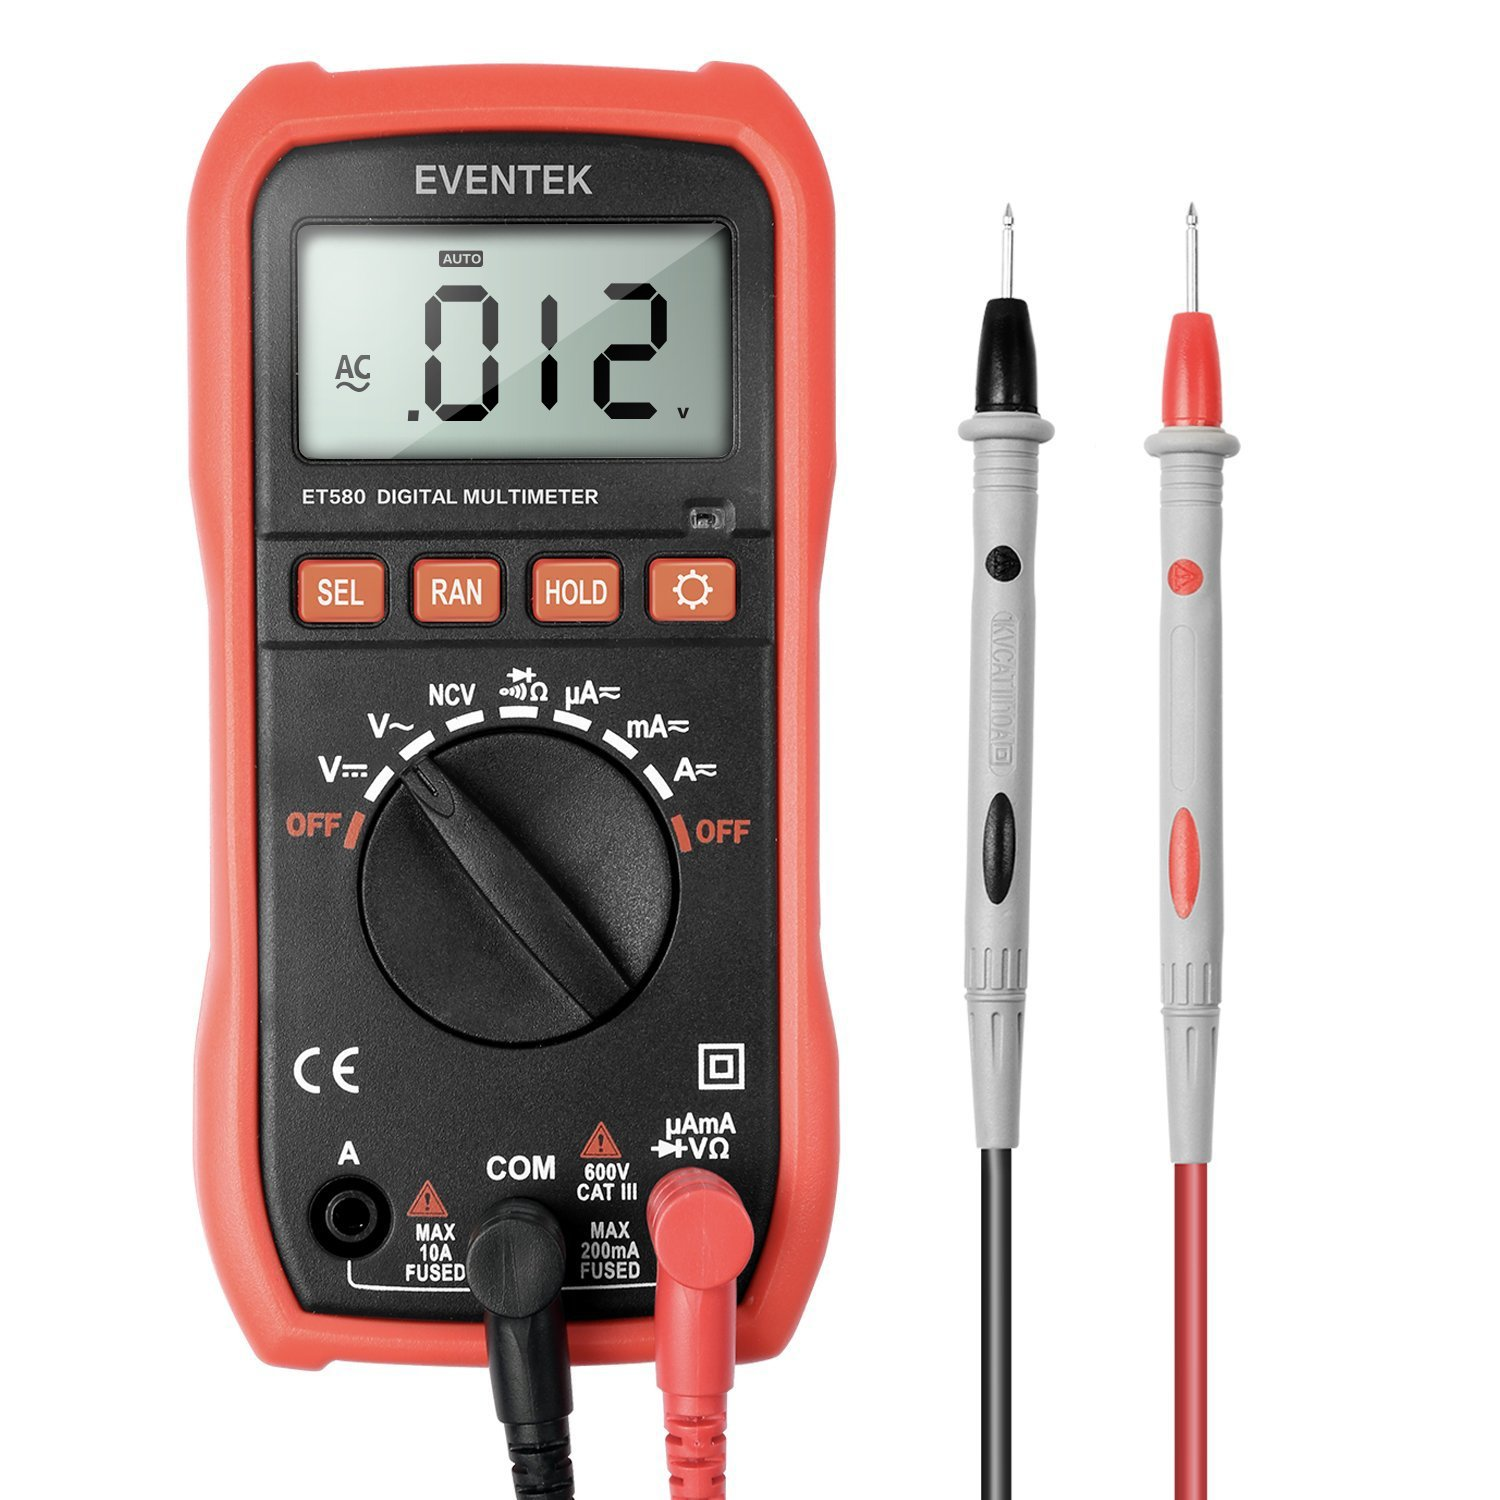
\includegraphics[width=0.65\textwidth]{multimetre01.jpg}
    \caption{Multimètre}
    \label{fig:multimetre}
\end{figure}



\end{itemize}















\section{Manipulation pratique}










\subsection{Montage}





Dans ce laboratoire, nous avons d'abord eu besoin de mesurer le courant avec l'oscilloscope et il a donc fallu brancher le générateur de fonctions à l'oscilloscope à l'aide d'un câble coaxial comme sur la figure \ref{fig:oscilloscopeGenerateur}

\begin{figure}%[H]
    \centering
    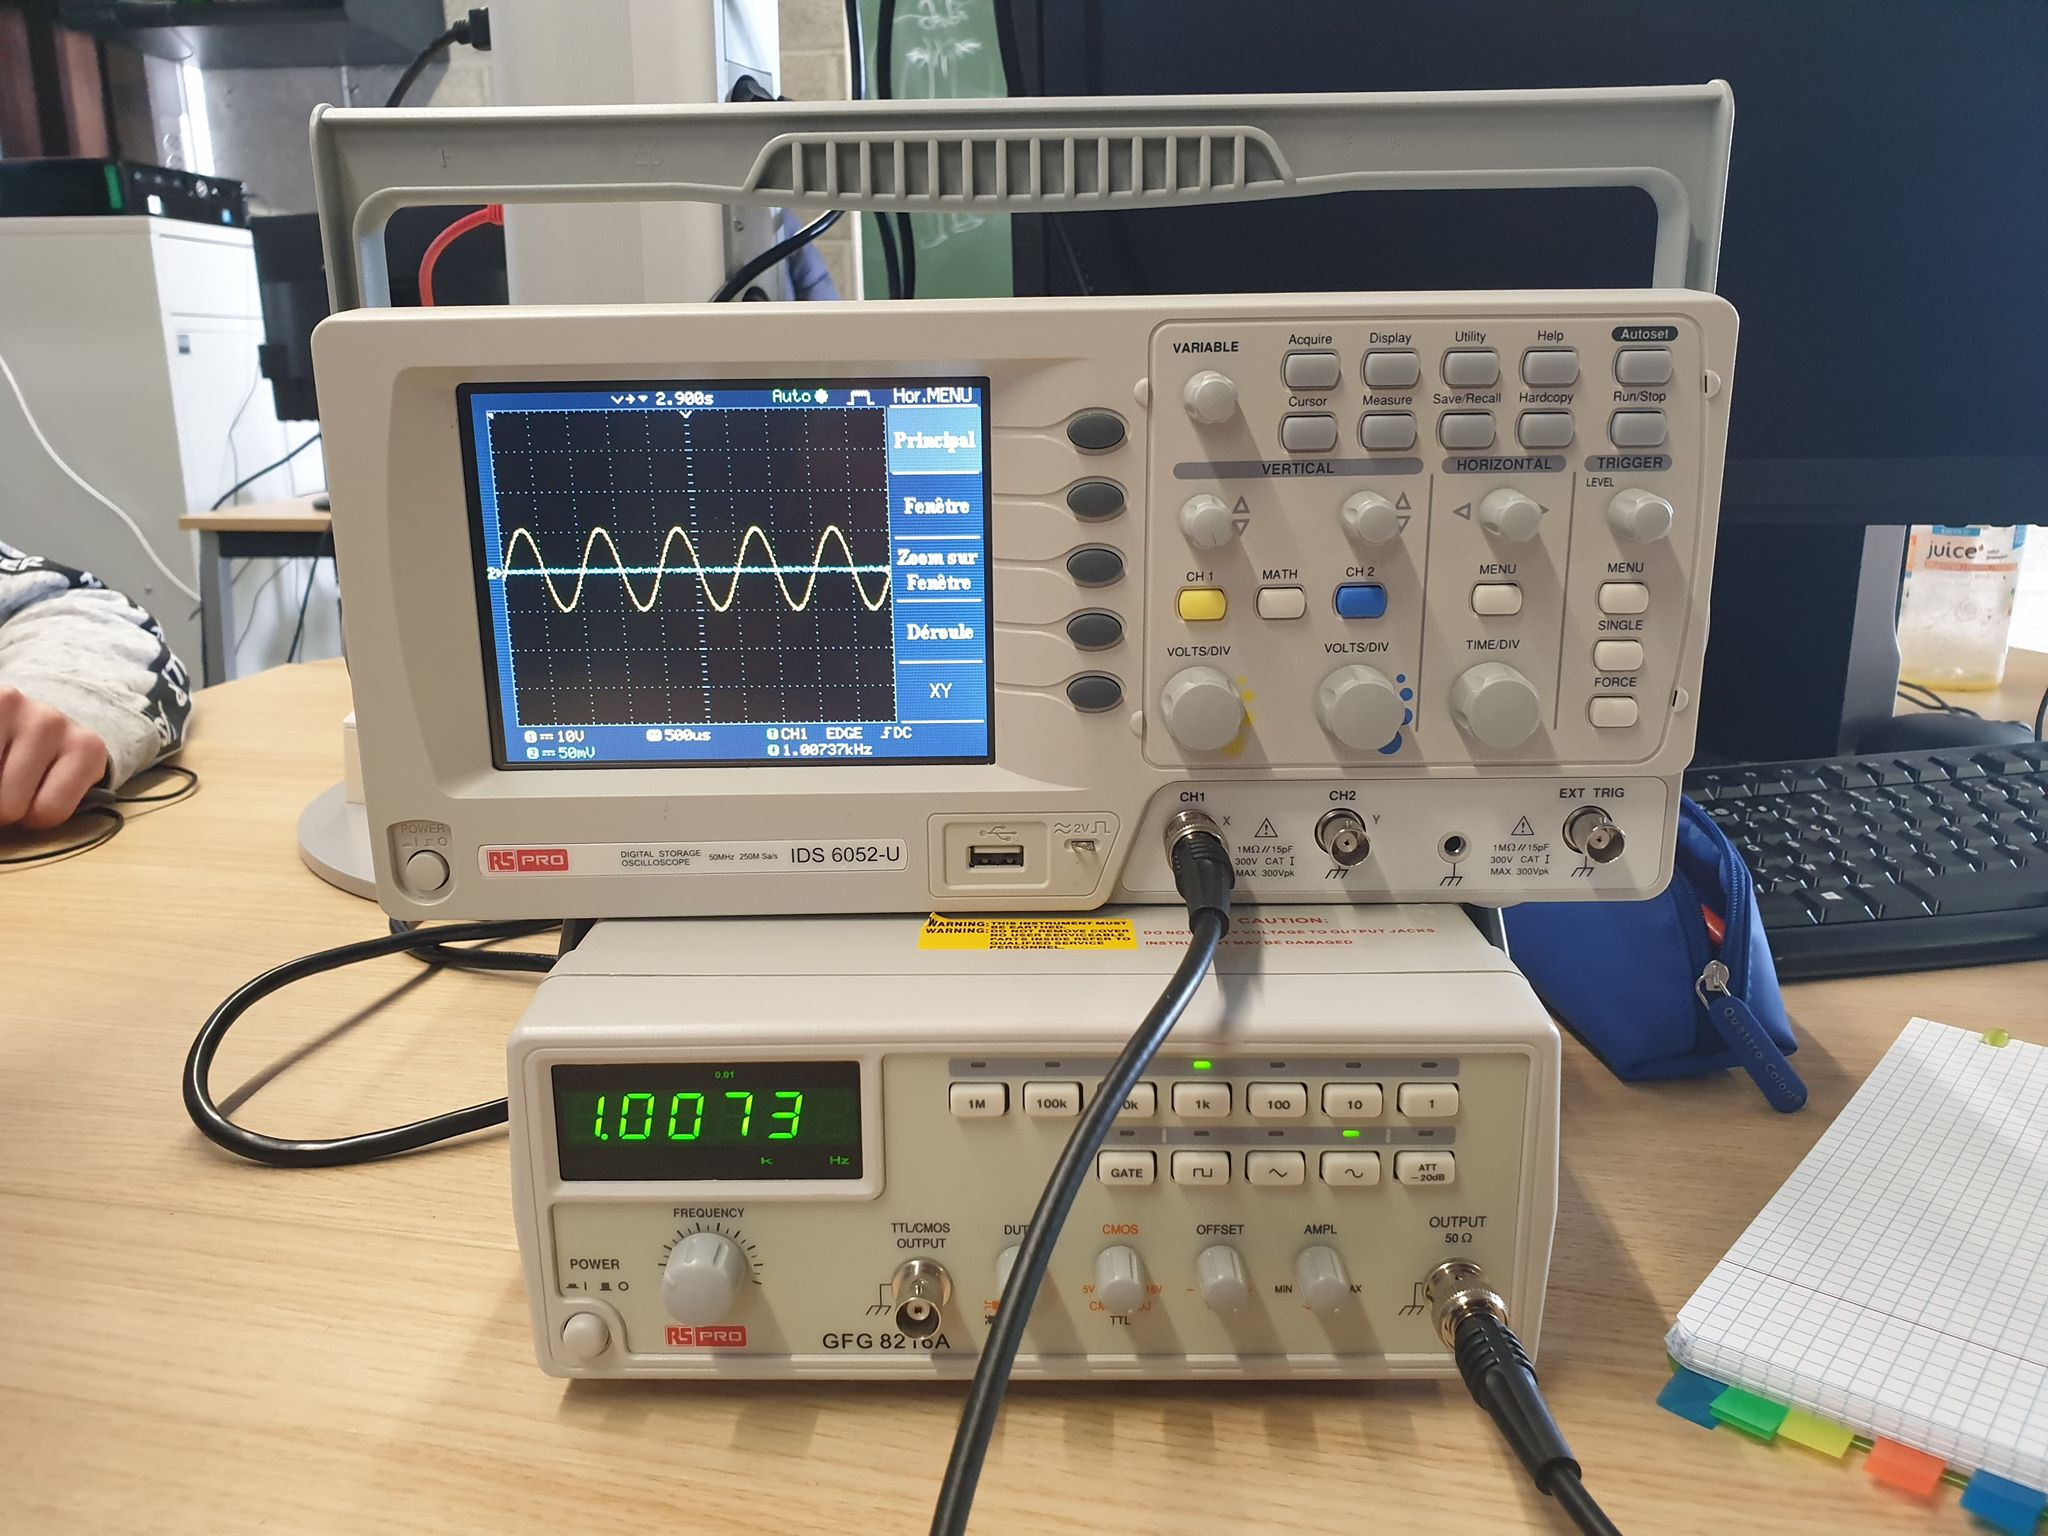
\includegraphics[width=0.95\textwidth]{oscilloscope-generateur.jpg}
    \caption{Oscilloscope connecté au générateur de fonction par un câble coaxial}
    \label{fig:oscilloscopeGenerateur}
\end{figure}










\subsection{Actions à effectuer}





Pour plus de clarté, nous avons copié l'énoncé de chaque étape en italique avant d'y répondre.

\begin{enumerate}





\item \textit{Générer un signal sinusoïdal d'1khz (d'amplitude max), sans atténuation. Visualiser correctement la forme sinusoïdale. Prouver que la fréquence est de 1Khz sur base de l'observation sur l'oscillo.}

% \begin{example}
  Afin de générer un signal d'un kilohertz, nous avons appuyé sur le bouton \textit{1k} du générateur de fonction. Ensuite, grâce à la manette \textit{Frequency}, nous avons essayé de rapprocher la valeur de la fréquence le plus possible de 1,0000 kHz. Nous sommes arrivés à obtenir 1,0045 kHz, soit une erreur absolue de 0,45 \% (voir figure \ref{fig:UnKhz02}). La lecture sur l'oscilloscope nous a donné une valeur de 1,004 kHz (voir figure \ref{fig:UnKhz03}).
% \end{example}

\begin{figure}%[H]
    \centering
    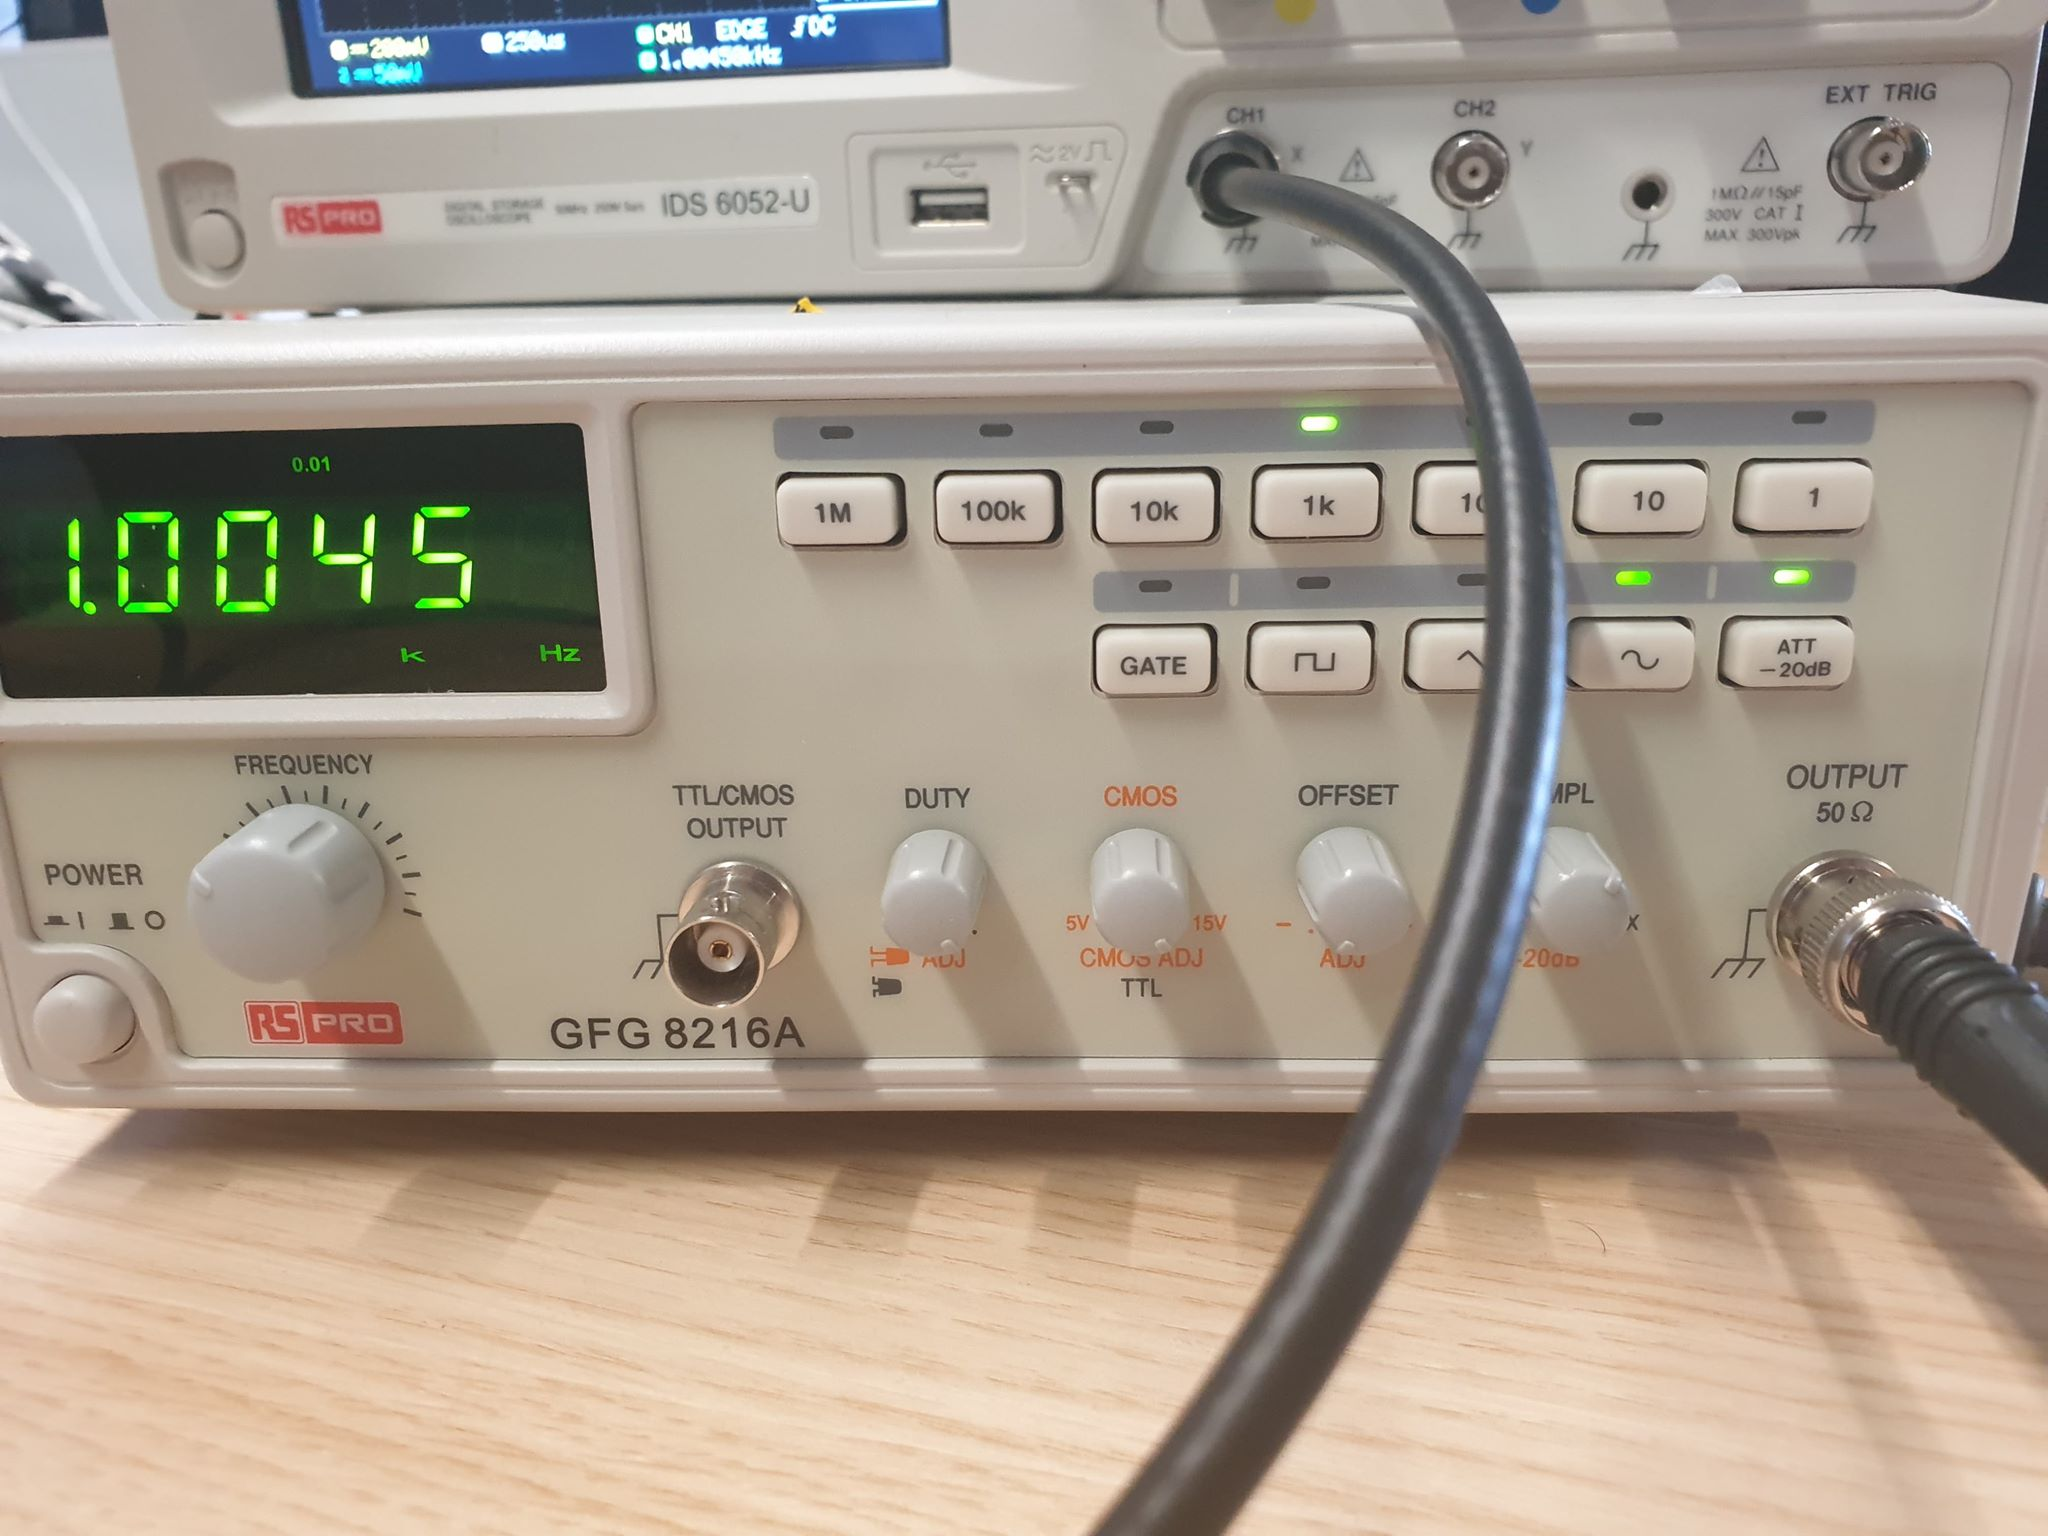
\includegraphics[width=0.75\textwidth]{UnKhz02.jpg}
    \caption{Lecture de la fréquence et de la tension sur le générateur de fonction}
    \label{fig:UnKhz02}
\end{figure}

\begin{figure}%[H]
    \centering
    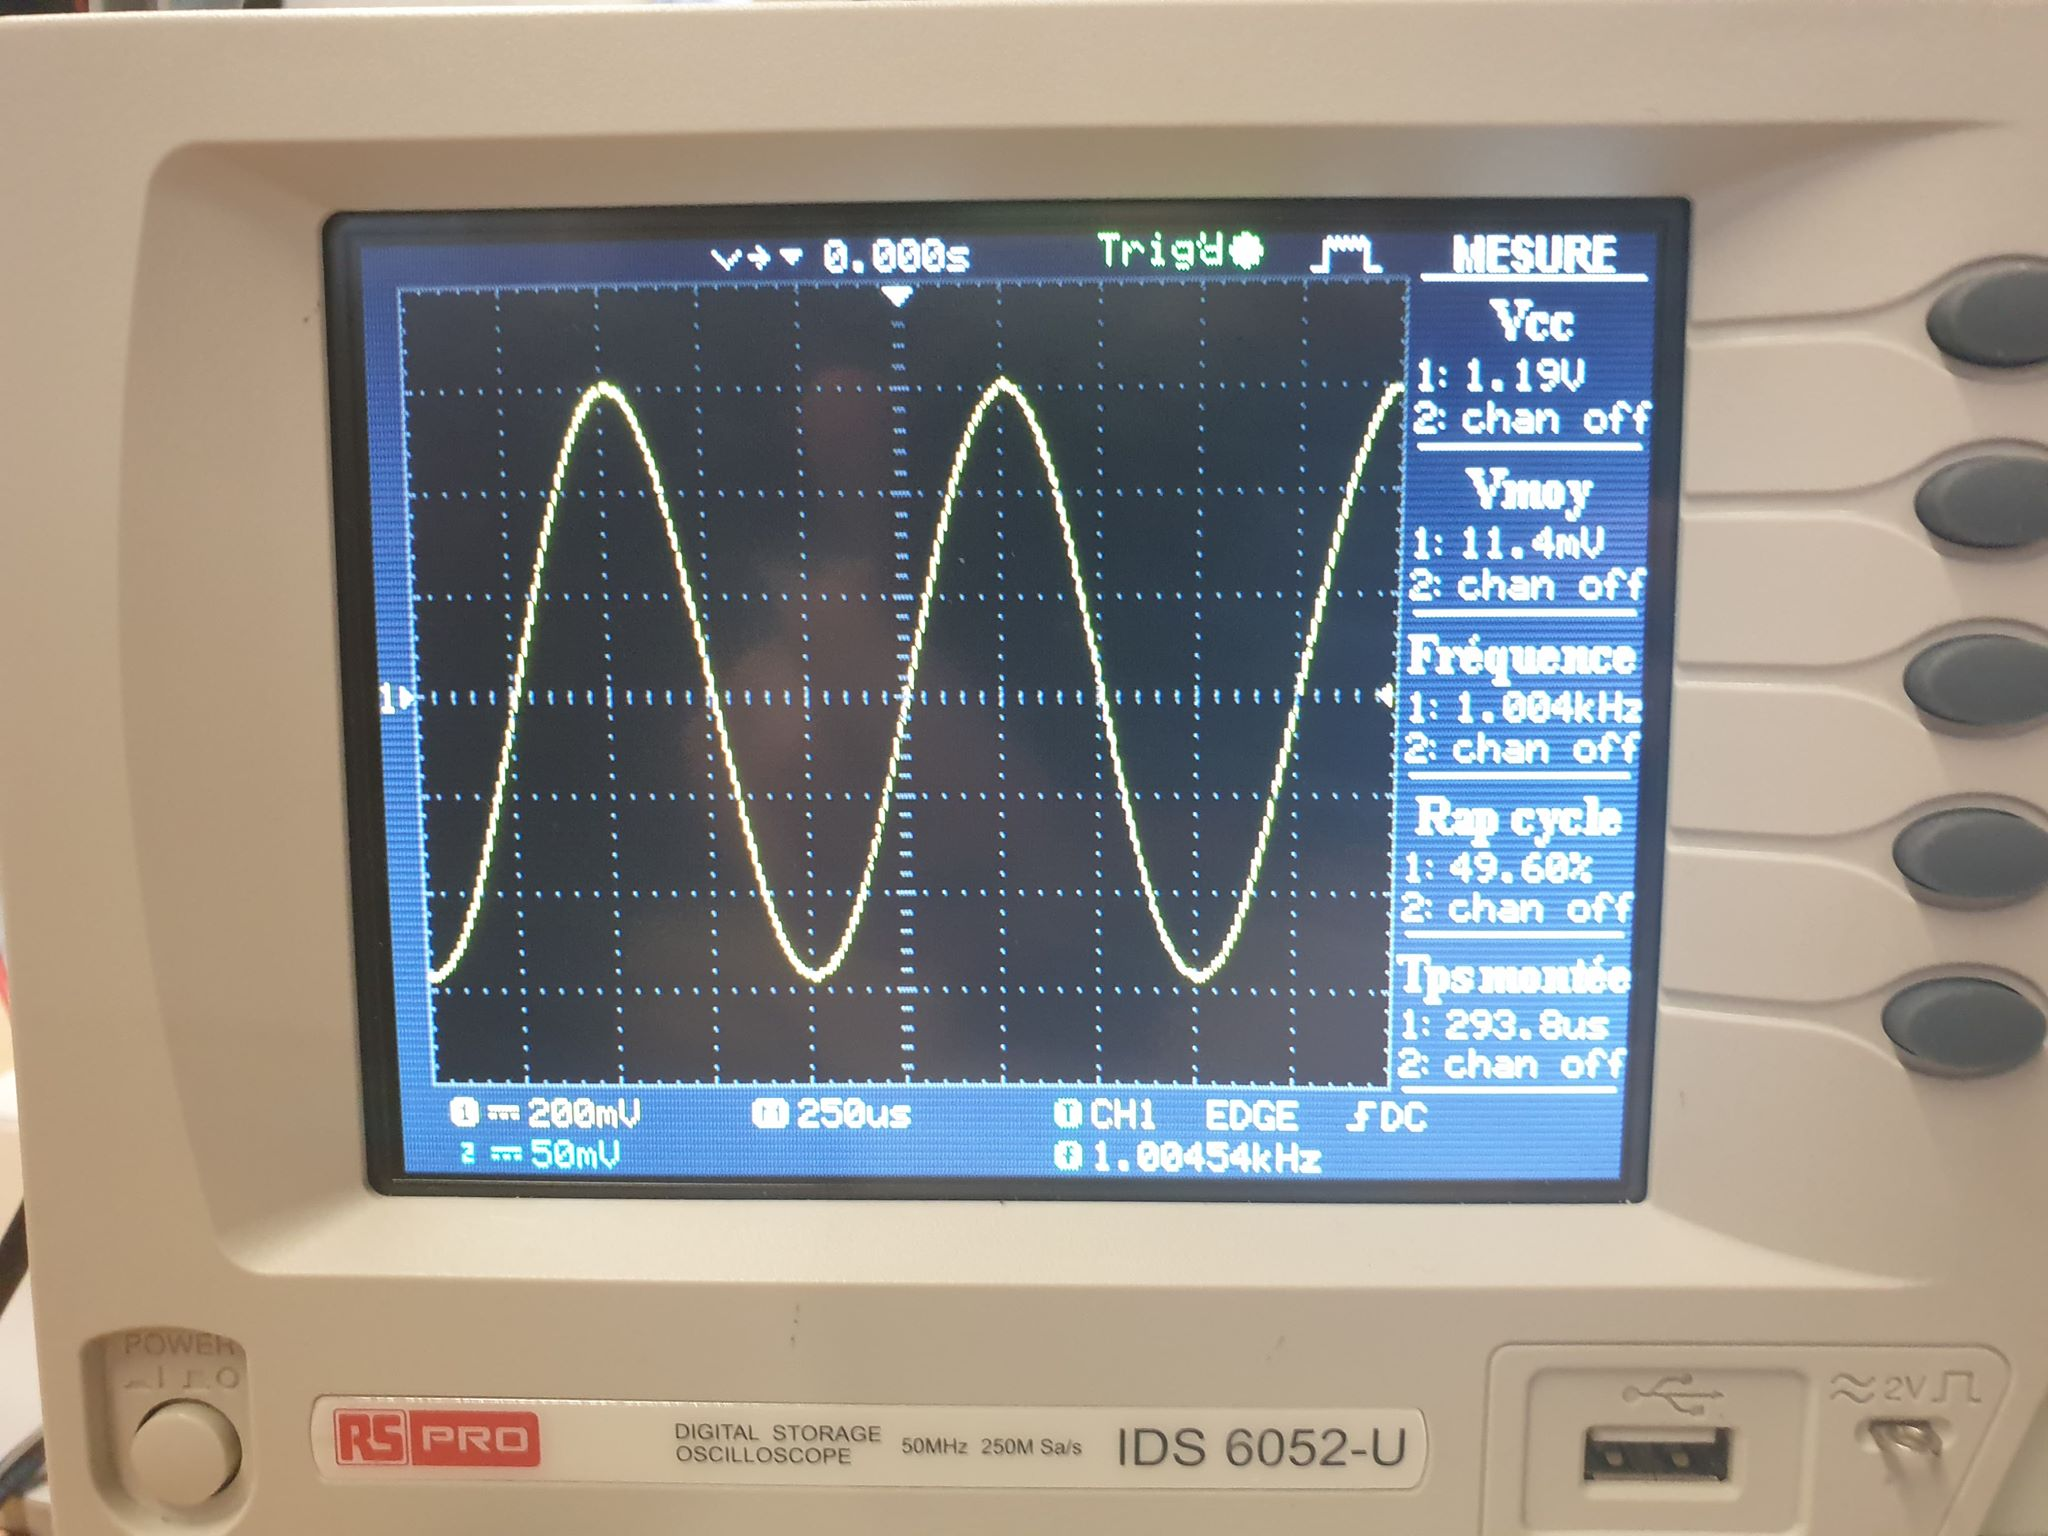
\includegraphics[width=0.75\textwidth]{UnKhz03.jpg}
    \caption{Lecture de la fréquence sur l'oscilloscope}
    \label{fig:UnKhz03}
\end{figure}





\item \textit{A l'aide d'un multimètre mesurer la tension. Comparer celle-ci avec l'observation de l'oscilloscope. Faire le lien avec les notions théoriques suivantes : Vmax, Veff.}

% \begin{example}
  Pour mesurer à l'aide du multimètre, il a fallu le mettre en contact avec le générateur de fonction, ce qui n'a pas été le plus évident pour nous dans cette manipulation. Pour le faire, nous avons connecté la sonde noire à la terre et la sonde rouge au courant (le courant sort du centre du port pour le câble coaxial). Le montage est illustré sur la figure \ref{fig:multimetreMesure}.
  
  Ensuite, nous avons réglé le multimètre en mode voltmètre, ce qui nous a permis de mesurer une tension. Mais cette tension était trop faible, de quelques millivolts seulement. En fait, nous mesurions la tension \textbf{moyenne} et pas la tension \textbf{efficace}. Pour mesurer la tension efficace, nous avons donc paramètré le multimètre, devenu voltmètre, en mode \textit{courant alternatif} et il a mesuré une tension efficace de \textbf{3,9 V}.

  Comme on peut le voir sur la figure \ref{fig:tensionOscilloscope}, l'oscilloscope nous donnait pour valeur de la tension crête à crête: $ V_{cc} = 11,4 $ V. Pour obtenir la valeur de la tension efficace, on va utiliser la formule:
  \[ V_{eff} = \frac{V_c}{\sqrt{2}} \]
  Puisque $ V_c $ (tension de crête) est le double de la tension crête à crête, le calcul devient:
  \[ V_{eff} = \frac{V_c}{\sqrt{2}} = \frac{V_{cc} / 2}{\sqrt{2}} = \frac{11,4 / 2}{\sqrt{2}} = 4,03 \; \text{V} \]
  Cette valeur est très proche de la tension efficace obtenue à l'aide du multimètre et est probablement due à des erreurs de mesure vu que le voltmètre est en série au lieu d'être en parallèle.

  \textbf{Remarque}: $ V_{max} = V_c $
% \end{example}

\begin{figure}%[H]
  \centering
  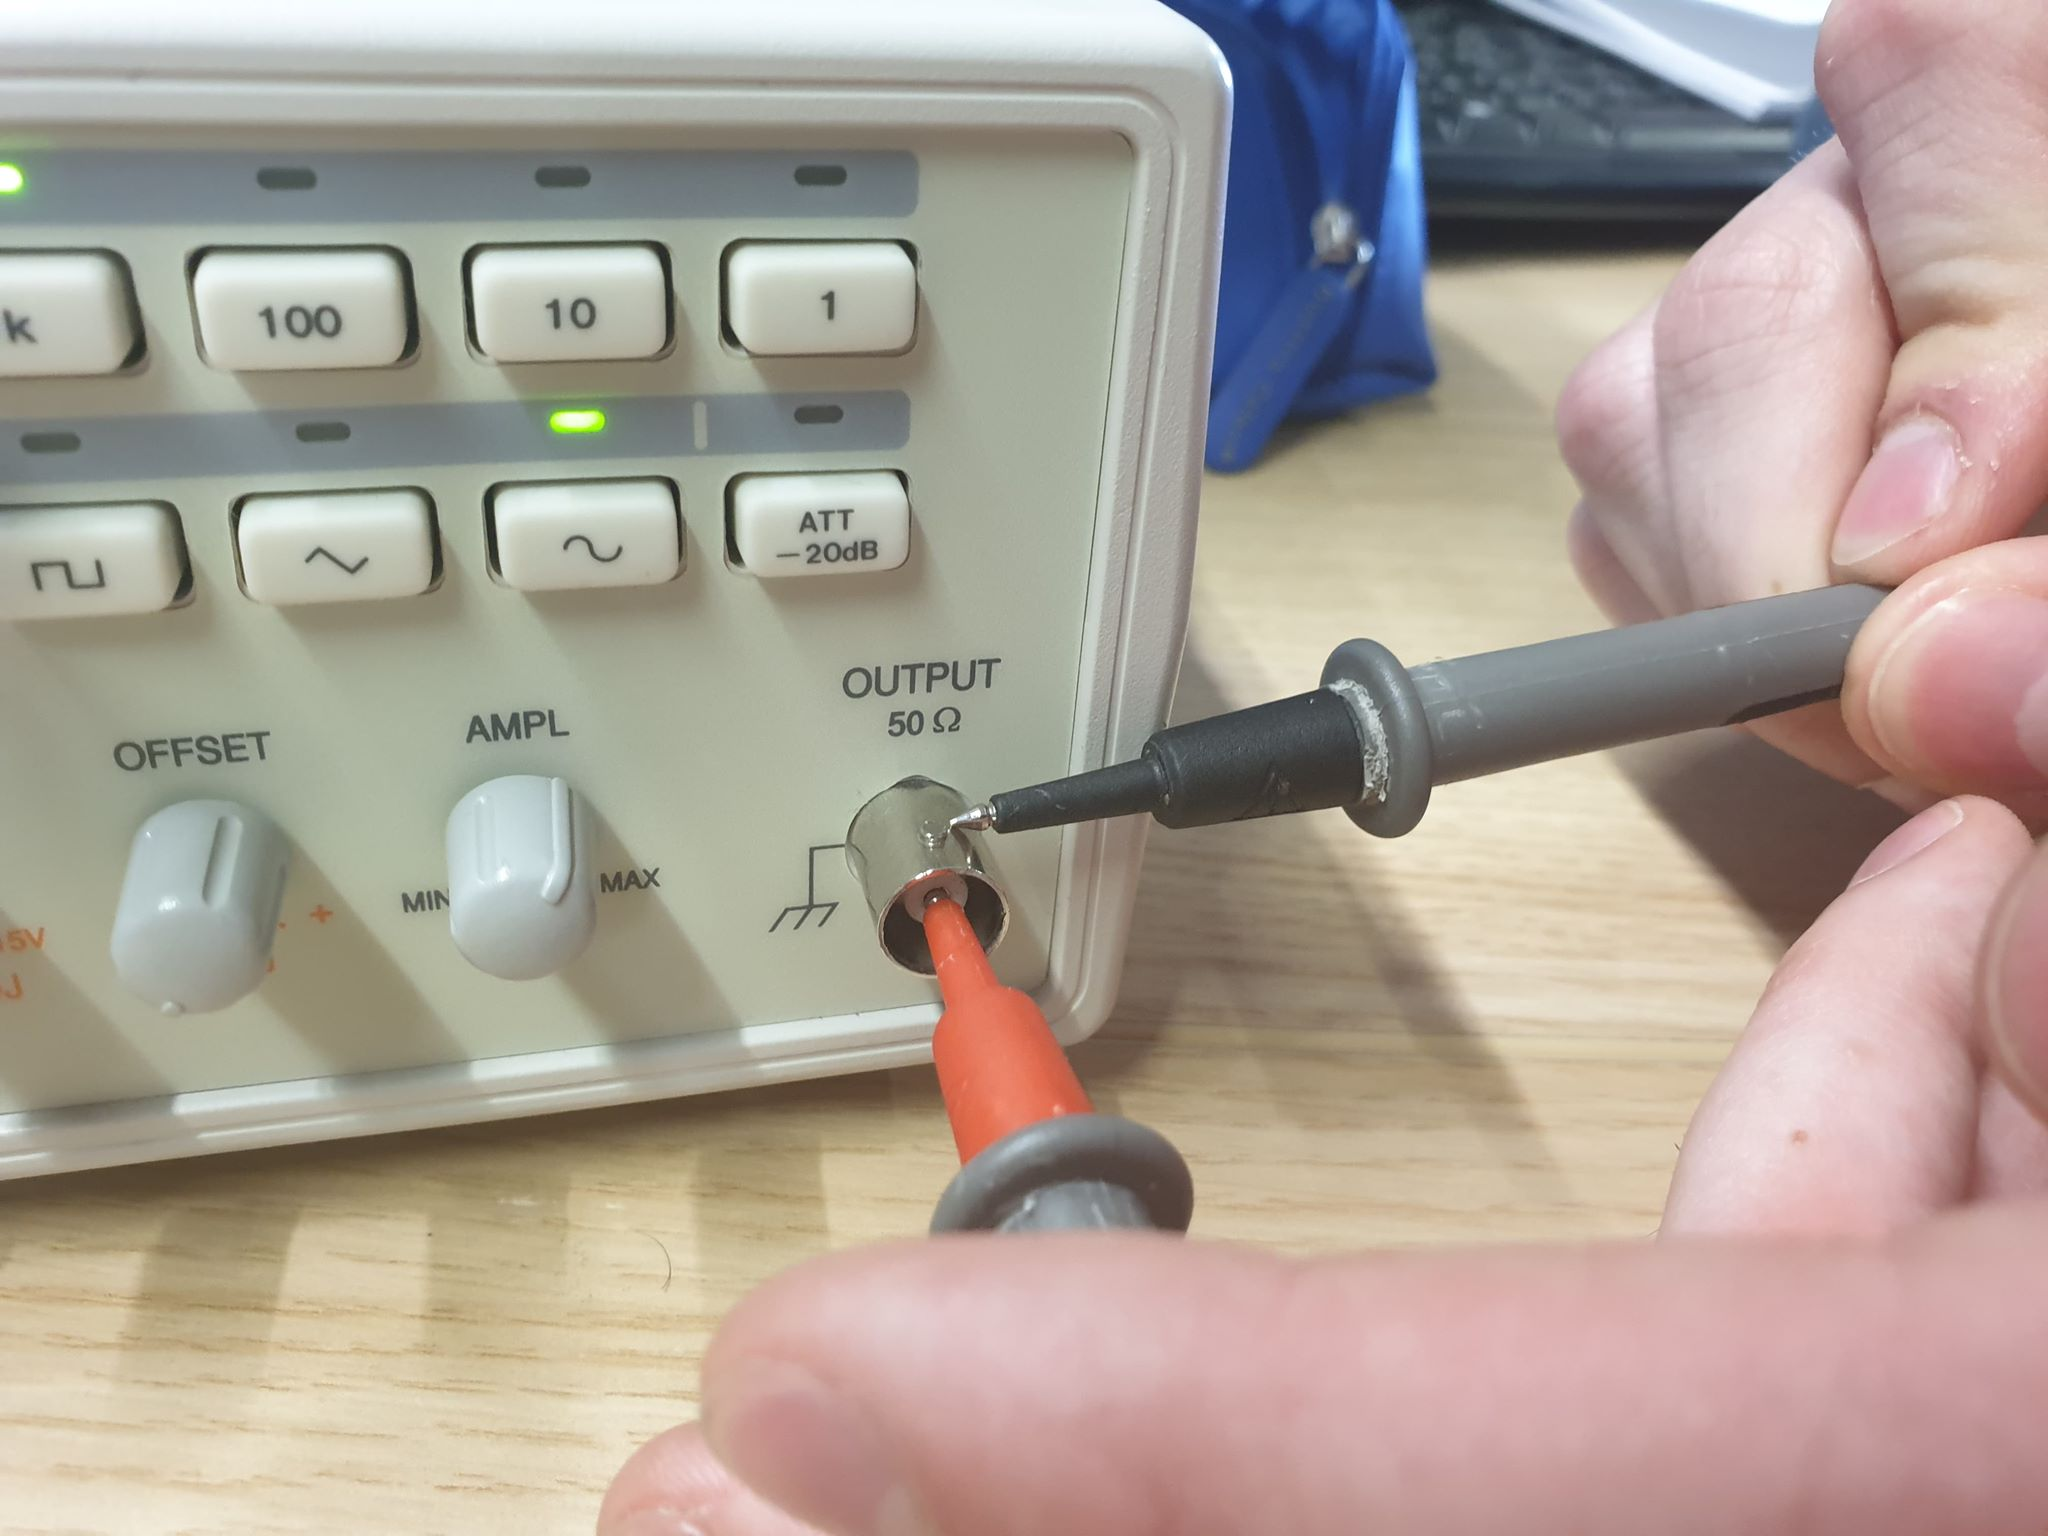
\includegraphics[width=0.75\textwidth]{multimetre-mesure01.jpg}
  \caption{Mesure de la tension à l'aide du multimètre}
  \label{fig:multimetreMesure}
\end{figure}

\begin{figure}%[H]
  \centering
  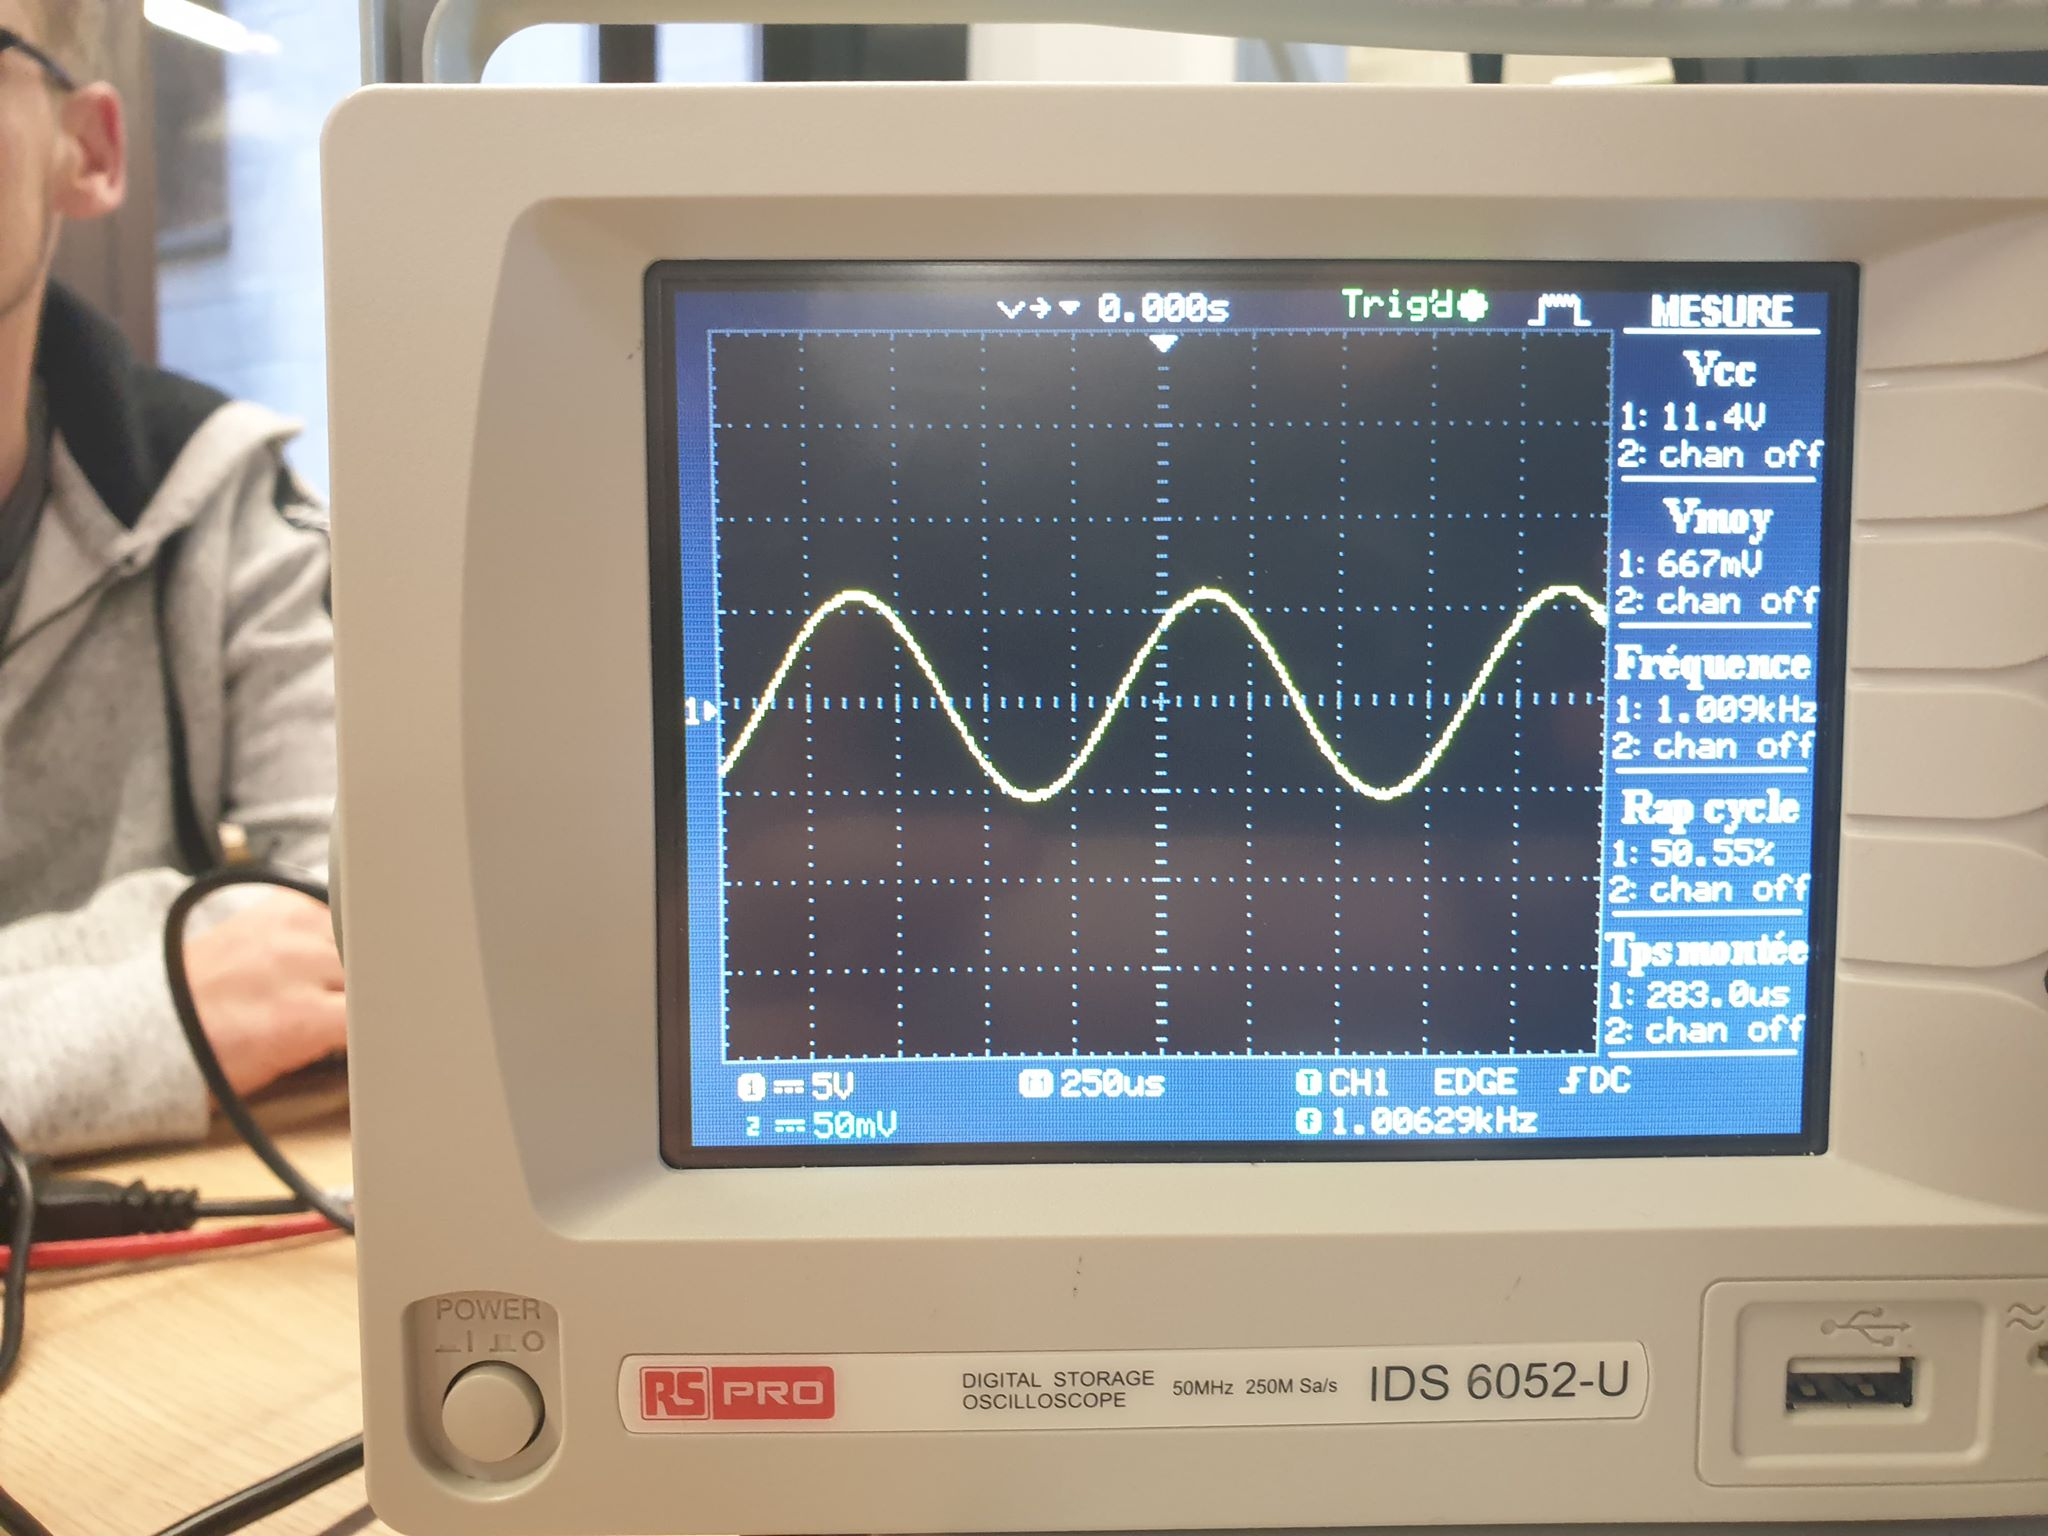
\includegraphics[width=0.95\textwidth]{tension-oscilloscope01.jpg}
  \caption{Mesure de la tension avec l'oscilloscope}
  \label{fig:tensionOscilloscope}
\end{figure}





\item \textit{Appuyer sur le bouton -20 dB et observer la nouvelle amplitude. Vérifier les observations avec la théorie (formules).}

% \begin{example}
  Comme on peut le voir sur la figure \ref{fig:UnKhz02}, une fois que l'on a mis un gain de -20 dB, la tension crête à crête mesurée par l'oscilloscope devient 1,19 V. Puisque nous avions mesuré une tension crête à crête de 11,4 V avant d'appliquer le gain, on peut calculer que la tension a été divisée par 9,58.

  D'un point de vue théorique, le gain est donné par:
  \[ G_{dB} = 10 \log \frac{P_S}{P_E} \]
  où $ P_S $ est la puissance du signal à la sortie de l'amplificateur et $ P_E $ est la puissance du signal à l'entrée de l'amplificateur. \\
  Si on applique un gain de -20 dB, la puissance du signal est donc divisée par 100:
  \[ -20 = 10 \log \frac{P_S}{P_E} \implies \frac{P_S}{P_E} = 10^{-2} \implies P_S = \frac{P_E}{100} \]
  
  Étant donné que la puissance est égale au produit de la tension et de l'intensité du courant, soit:
  \[ P = U \times I \]
  on en conclut que la tension et le courant sont tous deux divisés par 10 quand la puissance est divisée par 100. Ce qui correspond à peu près à la mesure sur l'oscilloscope, où nous avions mesuré que la tension de crête avait été divisée par 9,58.

% \end{example}





\item \textit{Expliquer à quoi sert le bouton "trigger".}

% \begin{example}
  Le bouton \textit{trigger} (déclencheur) est très important pour que le signal apparaisse de manière claire à l'écran. Il permet de synchroniser le balayage horizontal de l'oscilloscope en un point approprié, ce qui donne à l'onde une apparence statique.

  La variation de la tension de déclenchement et la différence entre le déclenchement pour un signal montant et un signal descendant sont illustrés sur les figures \ref{fig:trigger01} et \ref{fig:trigger02} \footnote{\texttt{https://www.electronics-notes.com/articles/test-methods/oscilloscope/} \\ \texttt{oscilloscope-trigger.php}}.
% \end{example}

\begin{figure}%[H]
  \centering
  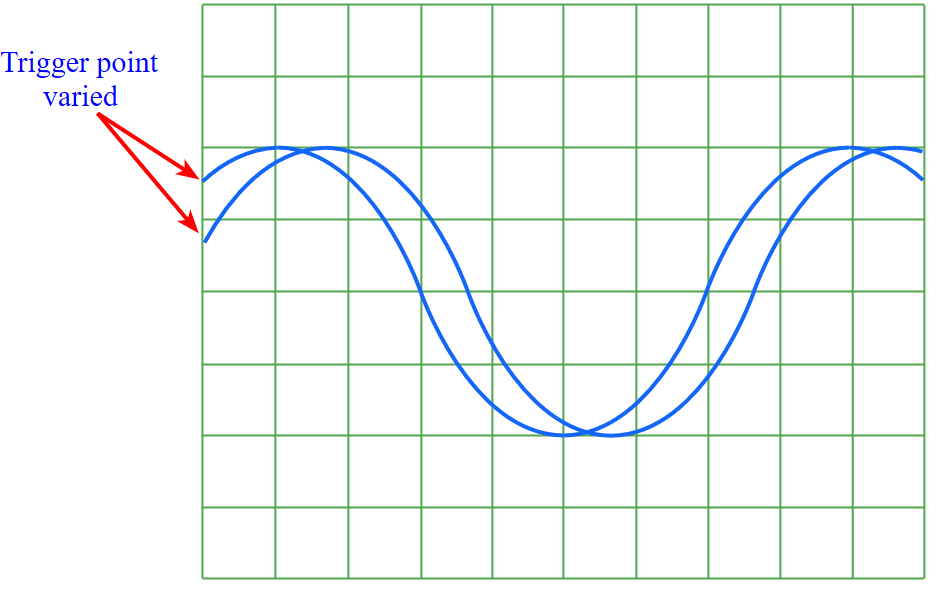
\includegraphics[width=0.75\textwidth]{trigger01.PNG}
  \caption{Variation de la tension de déclenchement}
  \label{fig:trigger01}
\end{figure}

\begin{figure}%[H]
  \centering
  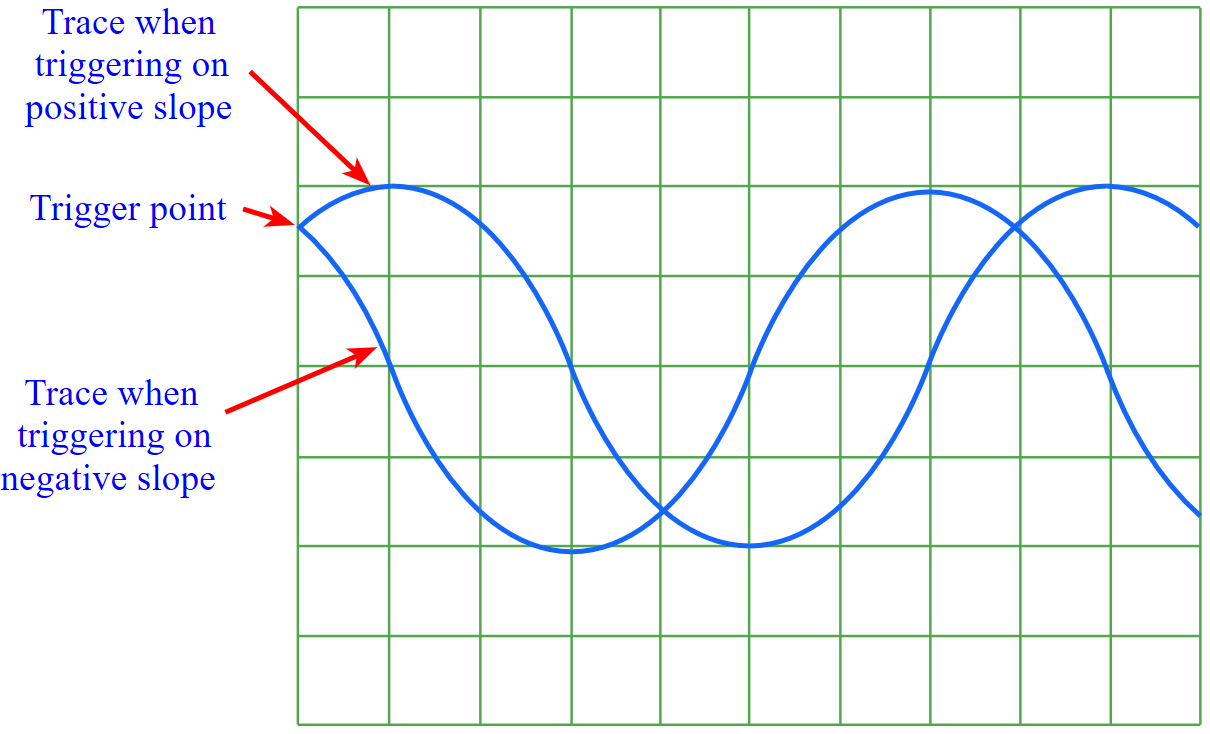
\includegraphics[width=0.75\textwidth]{trigger02.PNG}
  \caption{Déclenchement pour un signal montant et pour un signal descendant}
  \label{fig:trigger02}
\end{figure}





\item \textit{Générer un carré de 2Mhz, capturer sur l'oscilloscope.}

Nous avons réussi à générer un signal carré de 1,998 MHz. Pour cela, il a fallu changer la fréquence sur le générateur de fonction, ainsi que de clicker sur le bouton qui permet d'envoyer un signal carré au lieu d'un signal sinusoïdal ou triangulaire. On peut voir le signal capturé sur la figure \ref{fig:signalCarre2}

\begin{figure}%[H]
  \centering
  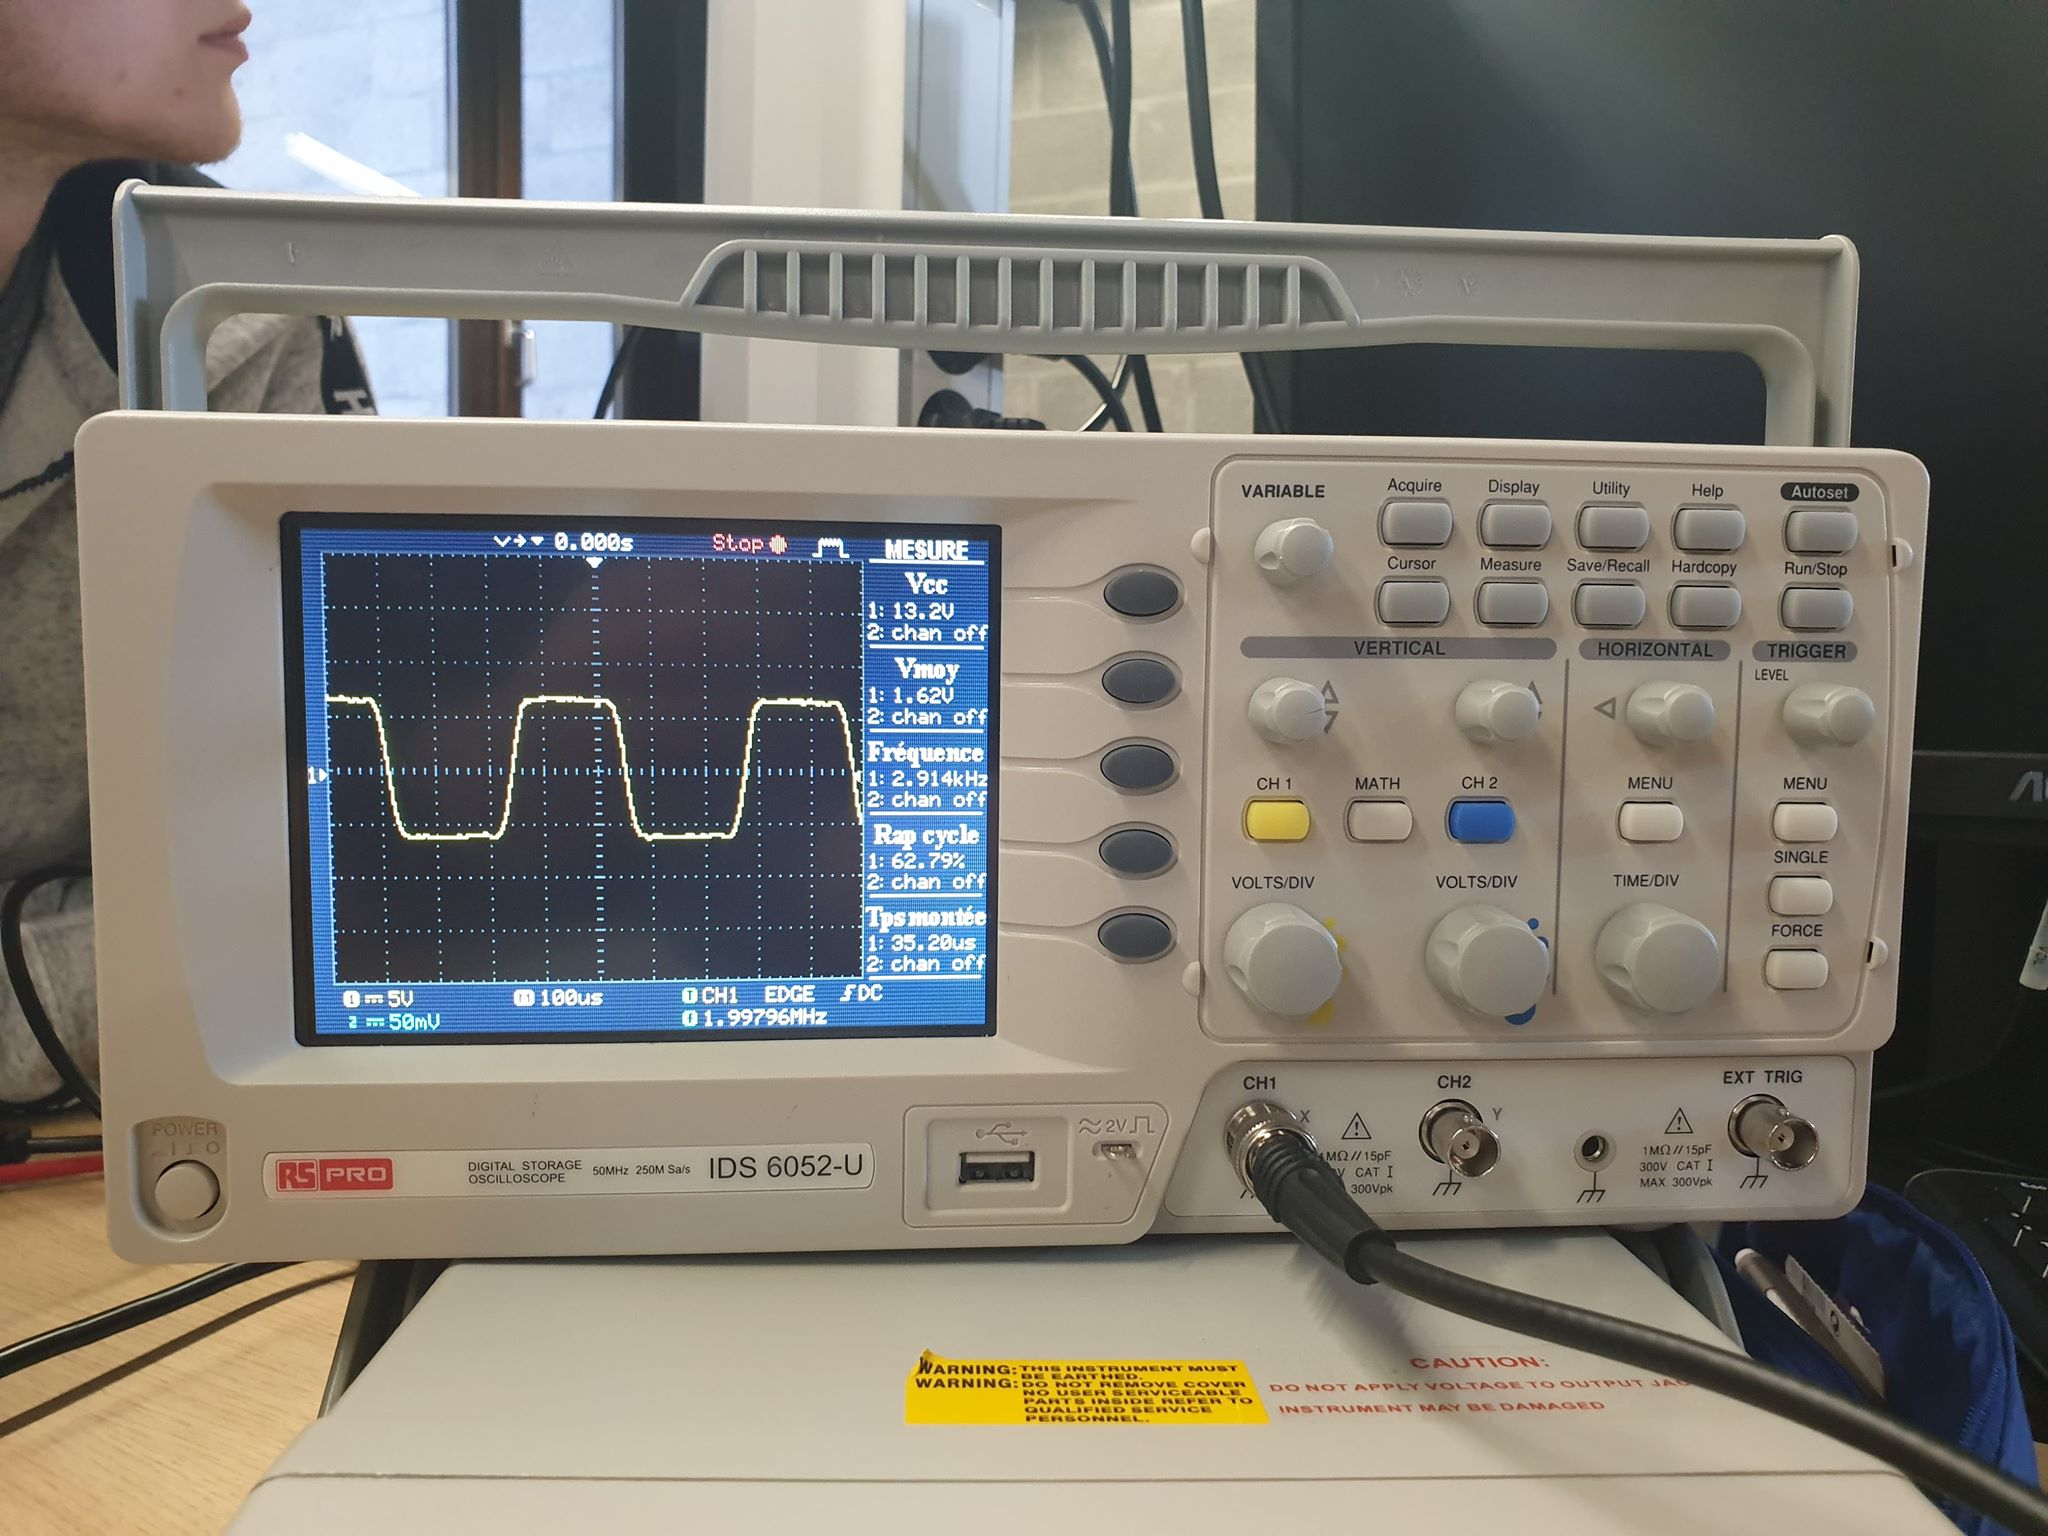
\includegraphics[width=0.95\textwidth]{signal-carre02.jpg}
  \caption{Signal carré de 2 MHz capturé sur l'oscilloscope.}
  \label{fig:signalCarre2}
\end{figure}





\item \textit{Descendre la fréquence à 200 Hz. Mesurer au multimètre la tension et la comparer avec l'oscilloscope. Faire le lien avec les notions théoriques suivantes : Vmax, Veff. Pourquoi est-ce nécessaire de diminuer la fréquence pour mesurer au multimètre ?}

%\begin{example}
  Après avoir descendu la fréquence de 2 MHz à 200 Hz, nous avons pris une photo de l'oscilloscope, vous pouvez la voir sur la figure \ref{fig:signalCarre1}. La tension crête à crête que l'on peut lire sur l'oscilloscope est de 13,4 V. Celle que nous avons mesuré avec le multimètre (comme sur la figure \ref{fig:multimetreMesure}) est la tension efficace et vaut 7,11 V.

  Pour un signal alternatif carré, la tension efficace est égale à la tension de crête. Dans ce cas-ci, on a:
  \[ V_{eff} = V_c = \frac{V_{cc}}{2} = \frac{13,4}{2} = 6,7 \; \text{V} \]
  Si on tient compte qu'il est plus facile de mesurer la tension avec l'oscilloscope qu'avec le multimètre, on peut conclure que l'erreur absolue de \textit{notre} mesure avec le multimètre est de 5,97 \%.

  La raison pour laquelle il faut diminuer la fréquence pour mesurer la tension avec le multimètre est que l'appareil n'est tout simplement pas adapté pour effectuer des mesures à des fréquences très élevées. Le multimètre est surtout utilisé par des électriciens sur des installations ou la fréquence est comprise entre 5 et 500 Hz. Pour des fréquences plus élevées, il faut utiliser un outil spécialisé comme un oscilloscope.
% \end{example}

\begin{figure}%[H]
  \centering
  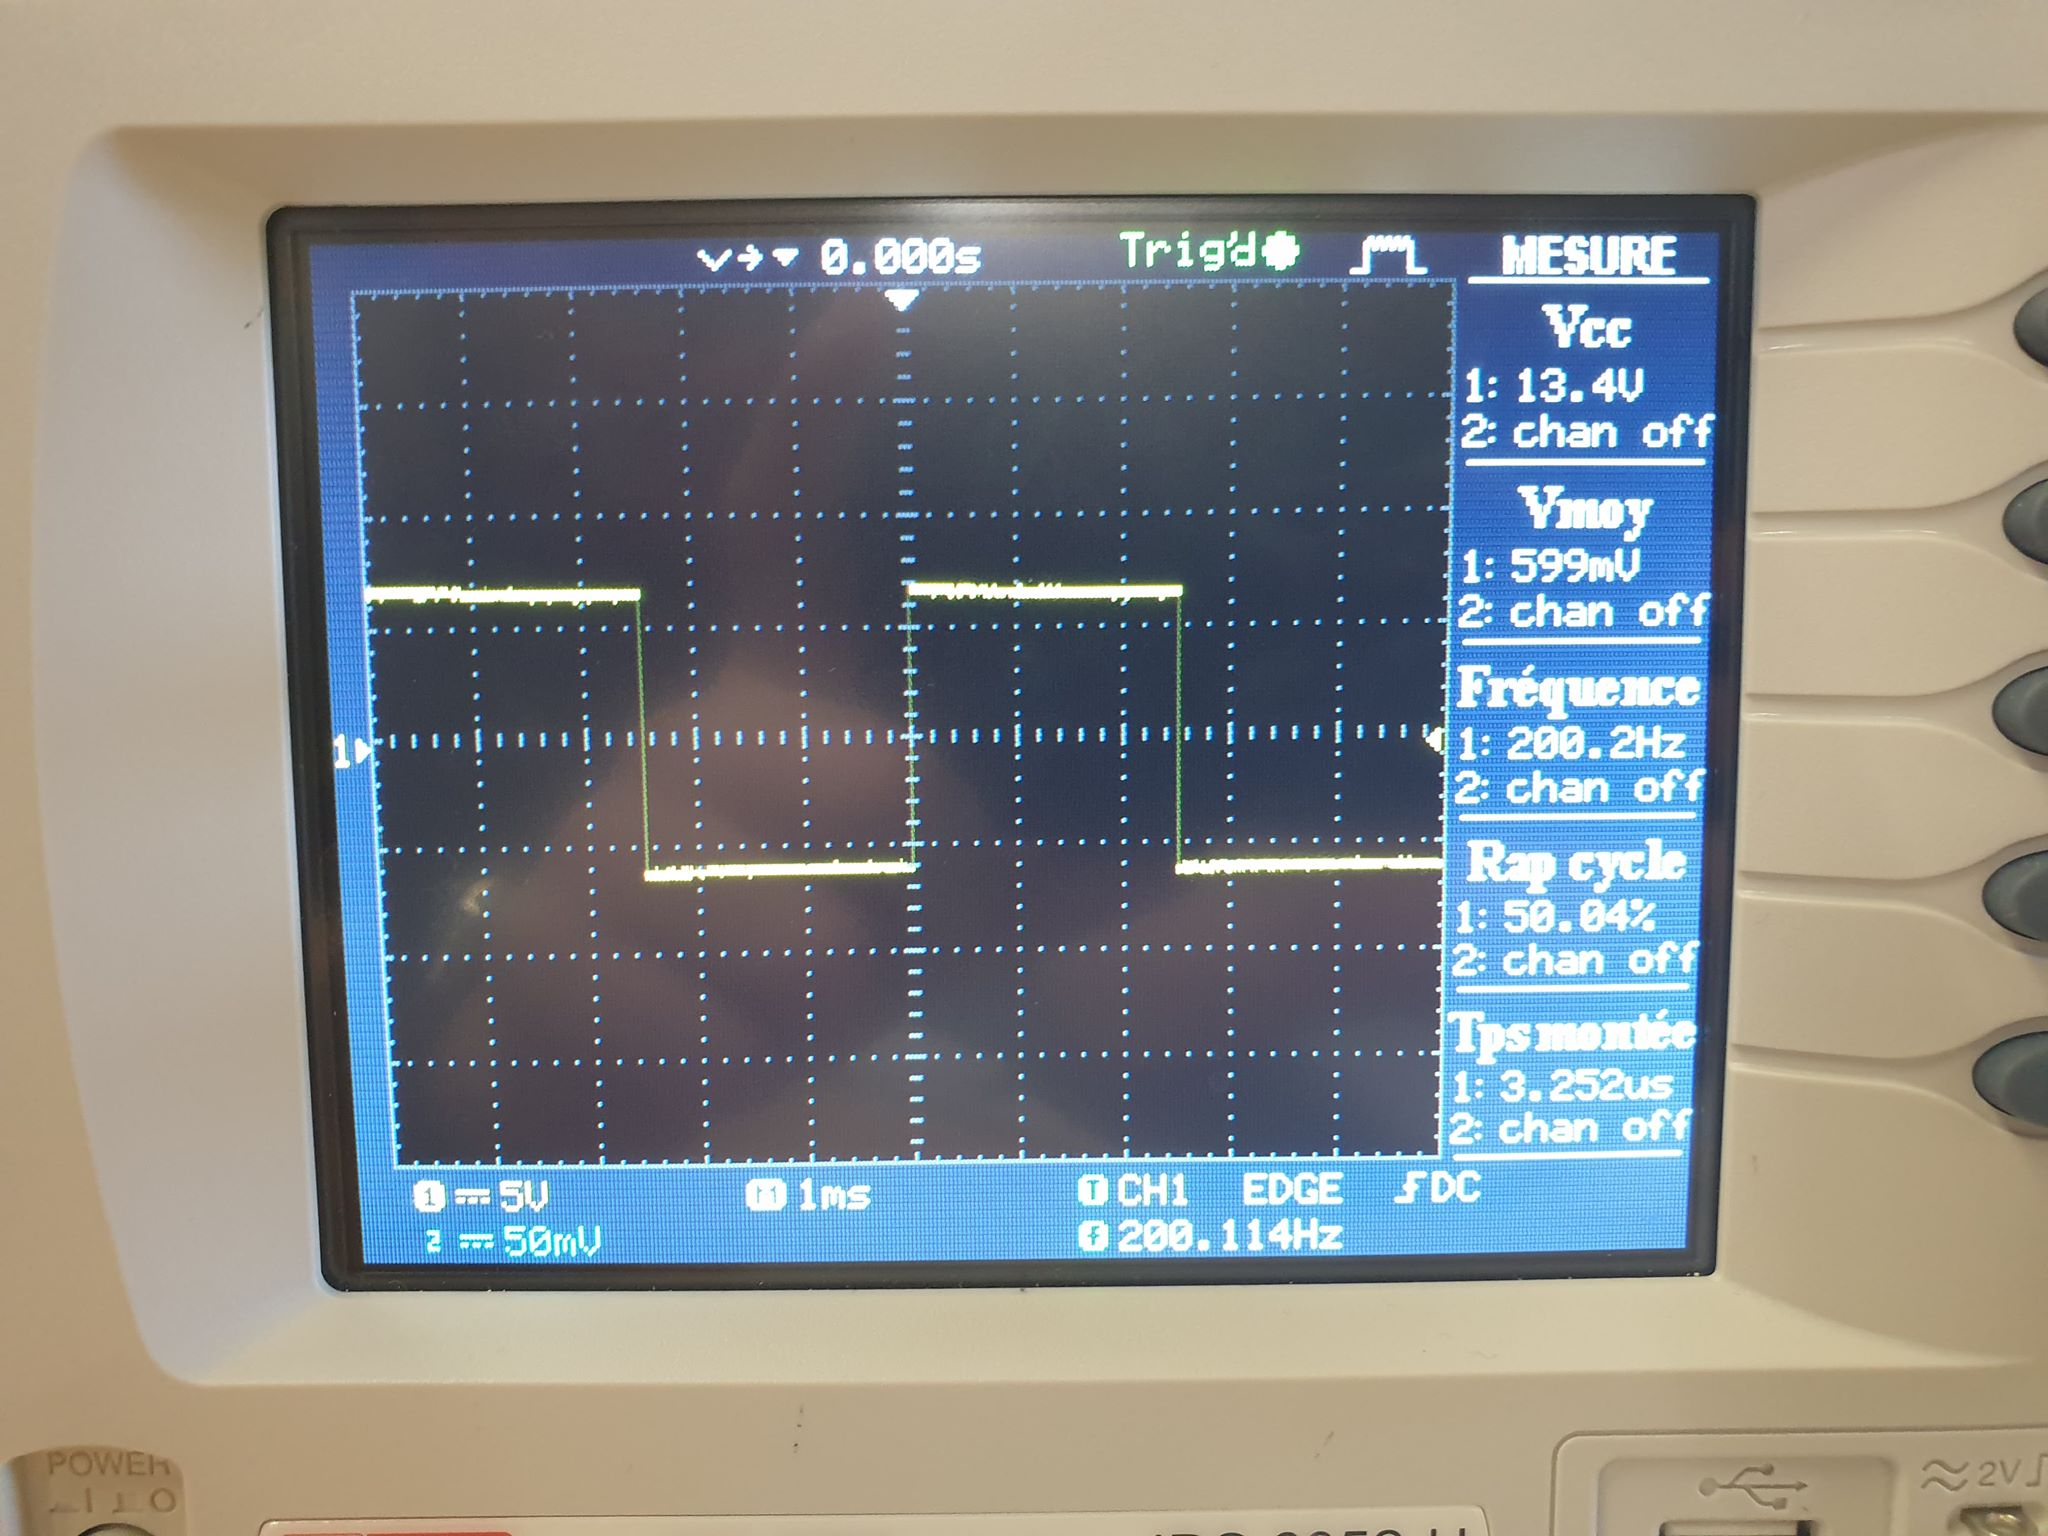
\includegraphics[width=0.75\textwidth]{signal-carre01.jpg}  
  \caption{Signal carré de 200 Hz capturé sur l'oscilloscope}
  \label{fig:signalCarre1}
\end{figure}





\end{enumerate}














\section{Conclusion}





En conclusion, nous avons appris à nous servir d’un multimètre lorsque l’on travaille avec des courants alternatifs. Nous savons dès à présent que lorsque le multimètre est réglé sur la tension pour un courant continu, celui-ci mesure en fait la tension moyenne $ V_{moy} $ de notre courant alternatif; et lorsqu’il est réglé pour la tension d’un courant alternatif, celui-ci nous donne la tension efficace $ V_{eff} $.

Nous avons aussi appris que lorsque l’on applique un gain de –20 dB a notre courant, $ V_{cc} $ est divisé par 10, exactement comme nous avons pu le constater sur l’oscilloscope (avec une minuscule marge d’erreur). 

Le bouton trigger, nous aura servi à voir qu’il est possible de synchroniser le balayage horizontal de l’oscilloscope en un point fixe et défini. 

Nous nous sommes aussi rendu compte que les multimètres ont leurs limites. En effet, au-dessus d’une certaine fréquence ($ \sim $ 500 Hz), les valeurs de ceux-ci deviennent imprécises, voir fausses et il est nécessaire d’utiliser un autre appareil de mesure tel qu’un oscilloscope.















\newpage \tableofcontents \listoffigures















\end{document}
